\documentclass[ignorenonframetext,]{beamer}
\setbeamertemplate{caption}[numbered]
\setbeamertemplate{caption label separator}{: }
\setbeamercolor{caption name}{fg=normal text.fg}
\beamertemplatenavigationsymbolsempty
\usepackage{lmodern}
\usepackage{amssymb,amsmath}
\usepackage{ifxetex,ifluatex}
\usepackage{fixltx2e} % provides \textsubscript
\ifnum 0\ifxetex 1\fi\ifluatex 1\fi=0 % if pdftex
  \usepackage[T1]{fontenc}
  \usepackage[utf8]{inputenc}
\else % if luatex or xelatex
  \ifxetex
    \usepackage{mathspec}
  \else
    \usepackage{fontspec}
  \fi
  \defaultfontfeatures{Ligatures=TeX,Scale=MatchLowercase}
\fi
\usetheme{AnnArbor}
\usecolortheme{dolphin}
\usefonttheme{professionalfonts}
% use upquote if available, for straight quotes in verbatim environments
\IfFileExists{upquote.sty}{\usepackage{upquote}}{}
% use microtype if available
\IfFileExists{microtype.sty}{%
\usepackage{microtype}
\UseMicrotypeSet[protrusion]{basicmath} % disable protrusion for tt fonts
}{}
\newif\ifbibliography
\usepackage{longtable,booktabs}
\usepackage{caption}
% These lines are needed to make table captions work with longtable:
\makeatletter
\def\fnum@table{\tablename~\thetable}
\makeatother
\usepackage{graphicx,grffile}
\makeatletter
\def\maxwidth{\ifdim\Gin@nat@width>\linewidth\linewidth\else\Gin@nat@width\fi}
\def\maxheight{\ifdim\Gin@nat@height>\textheight0.8\textheight\else\Gin@nat@height\fi}
\makeatother
% Scale images if necessary, so that they will not overflow the page
% margins by default, and it is still possible to overwrite the defaults
% using explicit options in \includegraphics[width, height, ...]{}
\setkeys{Gin}{width=\maxwidth,height=\maxheight,keepaspectratio}

% Prevent slide breaks in the middle of a paragraph:
\widowpenalties 1 10000
\raggedbottom

\AtBeginPart{
  \let\insertpartnumber\relax
  \let\partname\relax
  \frame{\partpage}
}
\AtBeginSection{
  \ifbibliography
  \else
    \let\insertsectionnumber\relax
    \let\sectionname\relax
    \frame{\sectionpage}
  \fi
}
\AtBeginSubsection{
  \let\insertsubsectionnumber\relax
  \let\subsectionname\relax
  \frame{\subsectionpage}
}

\setlength{\emergencystretch}{3em}  % prevent overfull lines
\providecommand{\tightlist}{%
  \setlength{\itemsep}{0pt}\setlength{\parskip}{0pt}}
\setcounter{secnumdepth}{0}


% \pgfdeclareimage[width=1cm]{logo}{./figures/monkeyTypewriter.png}
%\logo{\pgfuseimage{logo}}

\institute{University of Virginia}
\definecolor{links}{RGB}{42, 27, 129}
\definecolor{mypink2}{RGB}{219, 48, 122}
%\hypersetup{colorlinks,linkcolor=links,urlcolor=mypink2}
\usefonttheme{professionalfonts}

% \setbeamerfont{note page}{family*=pplx,size=\footnotesize} % Palatino for notes

\setbeamerfont{subtitle}{size=\small}

\definecolor{uvablue}{RGB}{0,85,150}
\definecolor{uvalibraryorange}{RGB}{252,175,23}
\definecolor{uvacream}{RGB}{241,229,199}
\definecolor{uvalightblue}{RGB}{163,220,230}

\setbeamercolor{block body}{bg=green,fg=green}
\setbeamercolor{block body alerted}{bg=green,fg=green}
\setbeamercolor{block body example}{bg=green,fg=green}

\setbeamercolor{caption name}{fg=uvablue}

\setbeamercolor{headline}{fg=uvacream,bg=uvacream}
\setbeamercolor{section}{fg=uvalibraryorange,bg=uvablue}
\setbeamercolor{frametitle}{fg=uvalibraryorange,bg=uvablue}
\setbeamercolor{palette primary}{bg=uvalibraryorange,fg=uvablue}
\setbeamercolor{palette secondary}{bg=uvablue,fg=uvablue}
\setbeamercolor{palette tertiary}{bg=uvalibraryorange,fg=uvablue}
\setbeamercolor{palette quarternary}{fg=uvalibraryorange,bg=uvablue}
\setbeamercolor{palette sidebar primary}{bg=uvalibraryorange,fg=uvablue}
\setbeamercolor{palette sidebar secondary}{fg=uvablue,bg=uvablue}
\setbeamercolor{palette sidebar tertiary}{fg=uvalibraryorange,bg=uvablue}
\setbeamercolor{palette sidebar quarternary}{fg=uvalibraryorange,bg=uvablue}
\setbeamercolor{structure}{bg=uvablue}



\useinnertheme{rectangles}

\titlegraphic{\vspace{-7.5mm}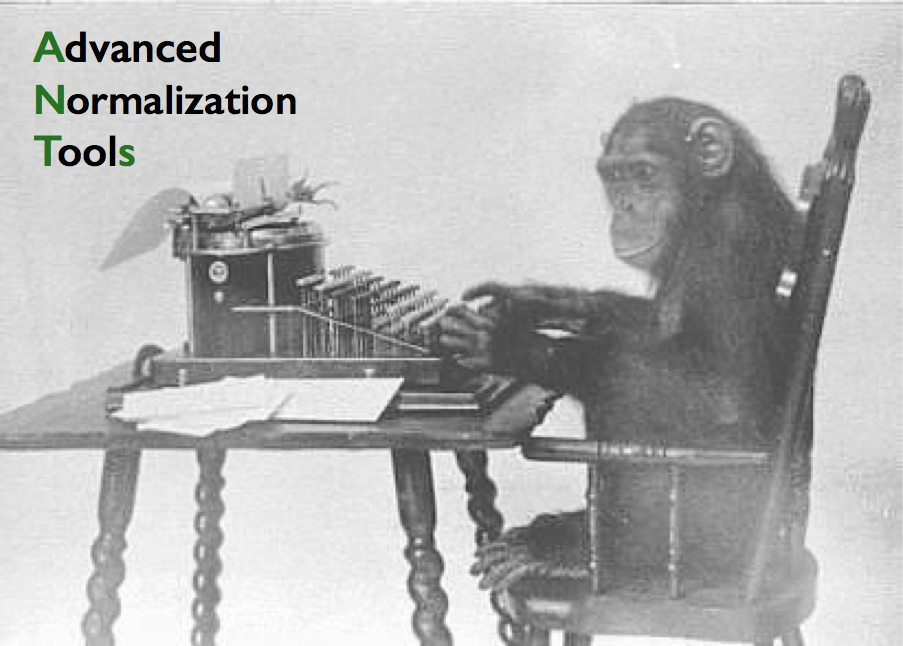
\includegraphics[width=0.45\paperwidth]{./figures/monkeyTypewriter.png}}

\title{ANTs Overview}
\author{Brian Avants and Nick Tustison}
\date{}

\begin{document}
\frame{\titlepage}

\section{Developers and
collaborators}\label{developers-and-collaborators}

\begin{frame}{Founders: Brian and Nick}

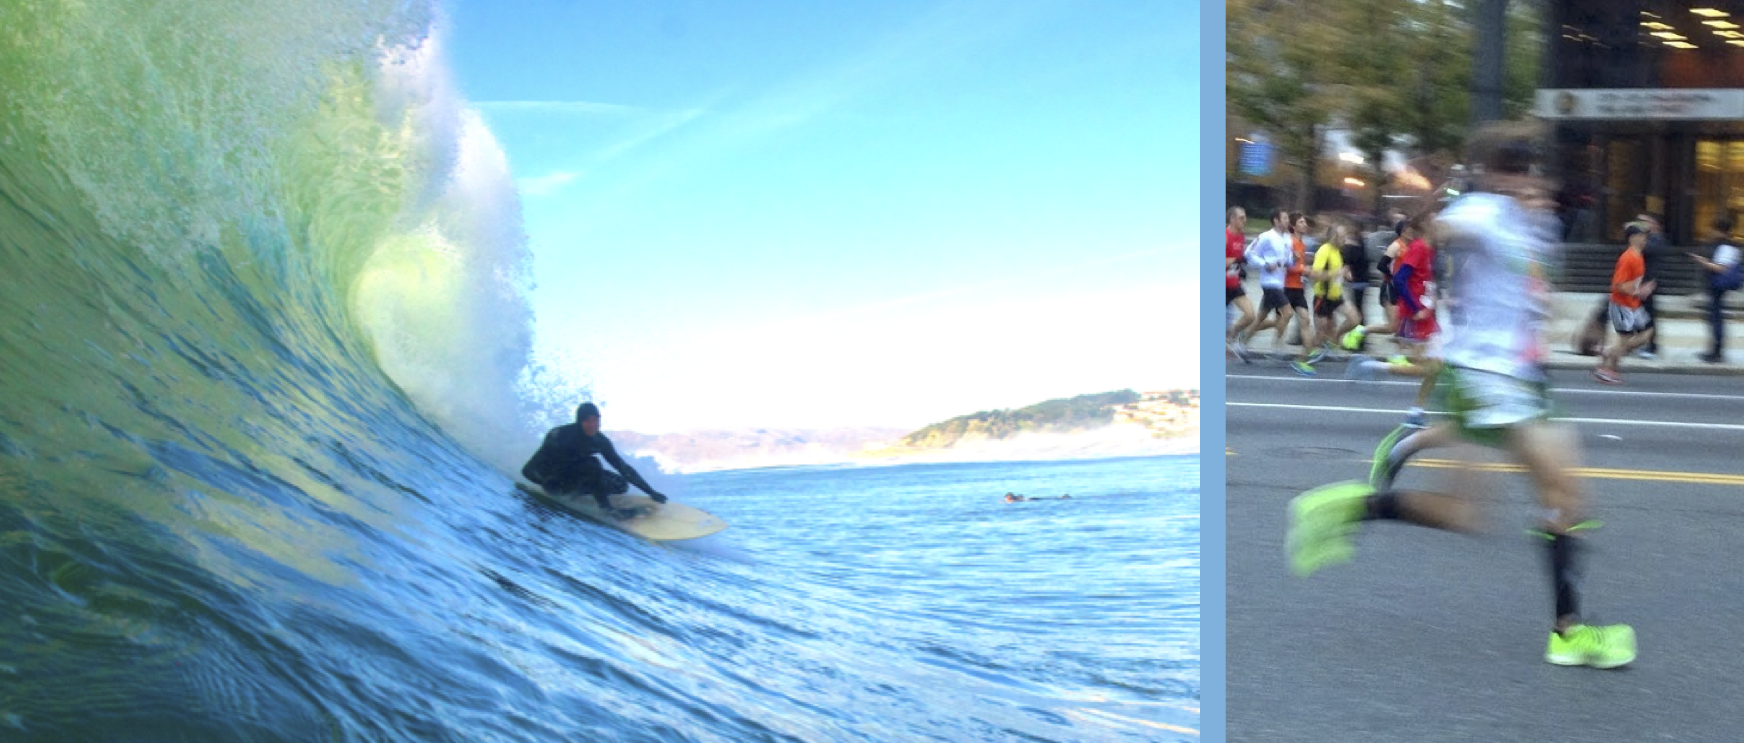
\includegraphics{./figures/brian_and_nick.png}

\end{frame}

\begin{frame}

\includegraphics{./figures/antsCollaborators2.png}

\(+\) \href{http://neuro.debian.net/pkgs/ants.html}{neurodebian},
\href{http://www.slicer.org/}{slicer},
\href{https://github.com/BRAINSia/BRAINSTools}{brainsfit},
\href{http://nipy.sourceforge.net/nipype/}{nipype},
\href{http://www.itk.org}{itk} and more \ldots{}

\end{frame}

\section{ANTs lineage}\label{ants-lineage}

\begin{frame}{Initial scope}

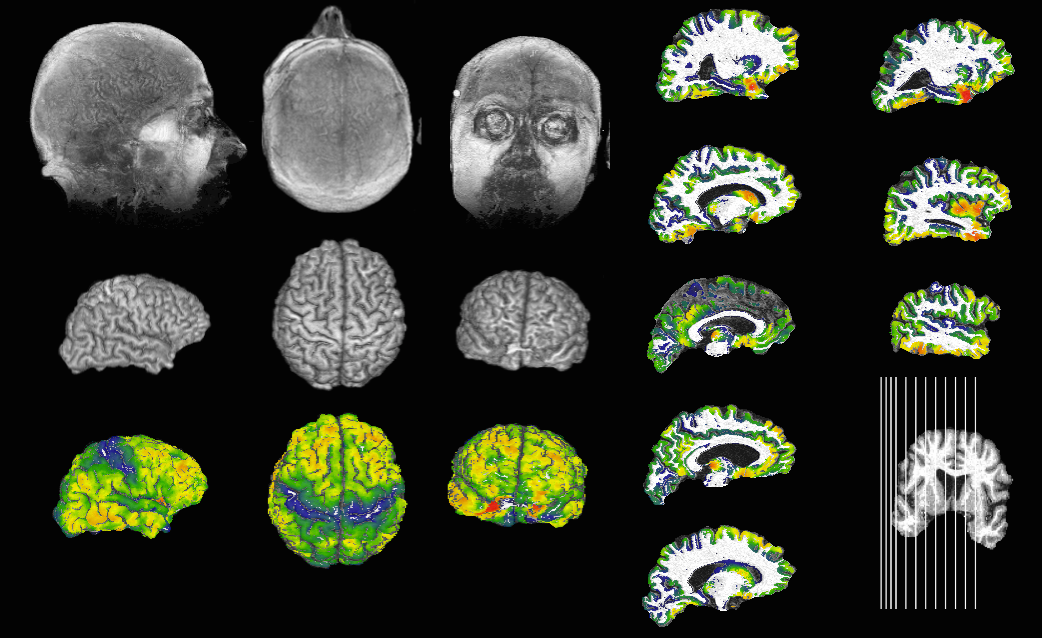
\includegraphics{./figures/ants_initial_scope.png}

\end{frame}

\section{Major ANTs utilities}\label{major-ants-utilities}

\begin{frame}{Donoho?}

 \emph{``Papers are just advertisements for the science.''}

\end{frame}

\begin{frame}{Neuro tools}

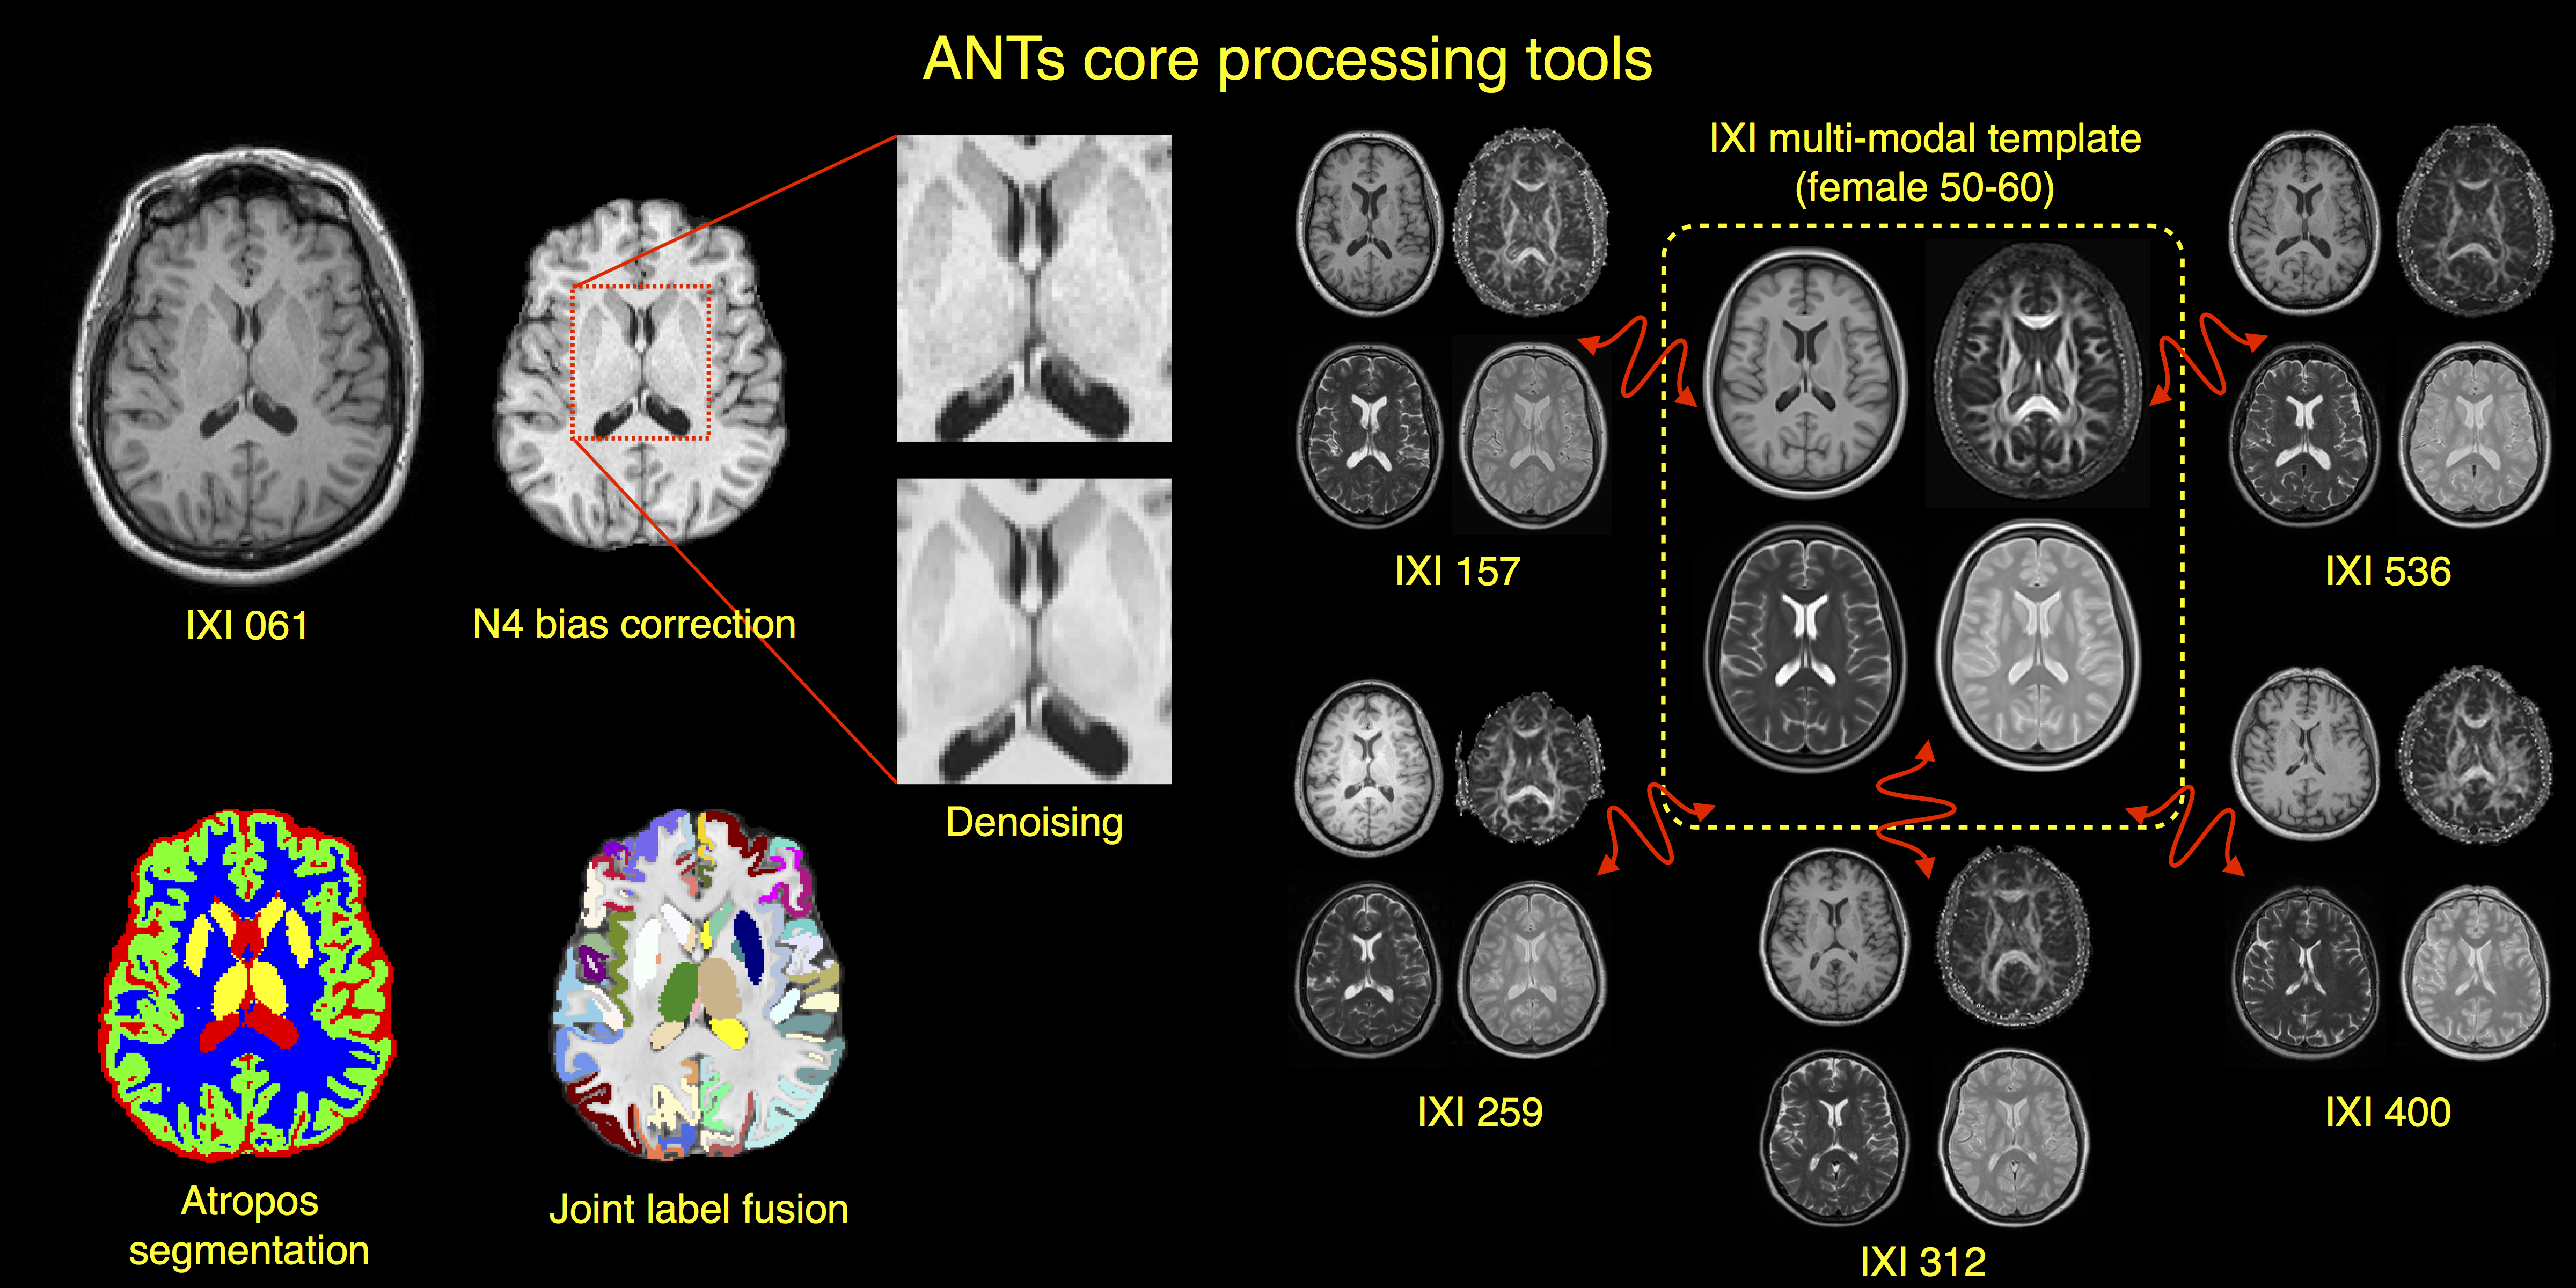
\includegraphics{./tools/figures/coreANtsToolsNeuro.png}

\end{frame}

\begin{frame}{Pulmonary tools}

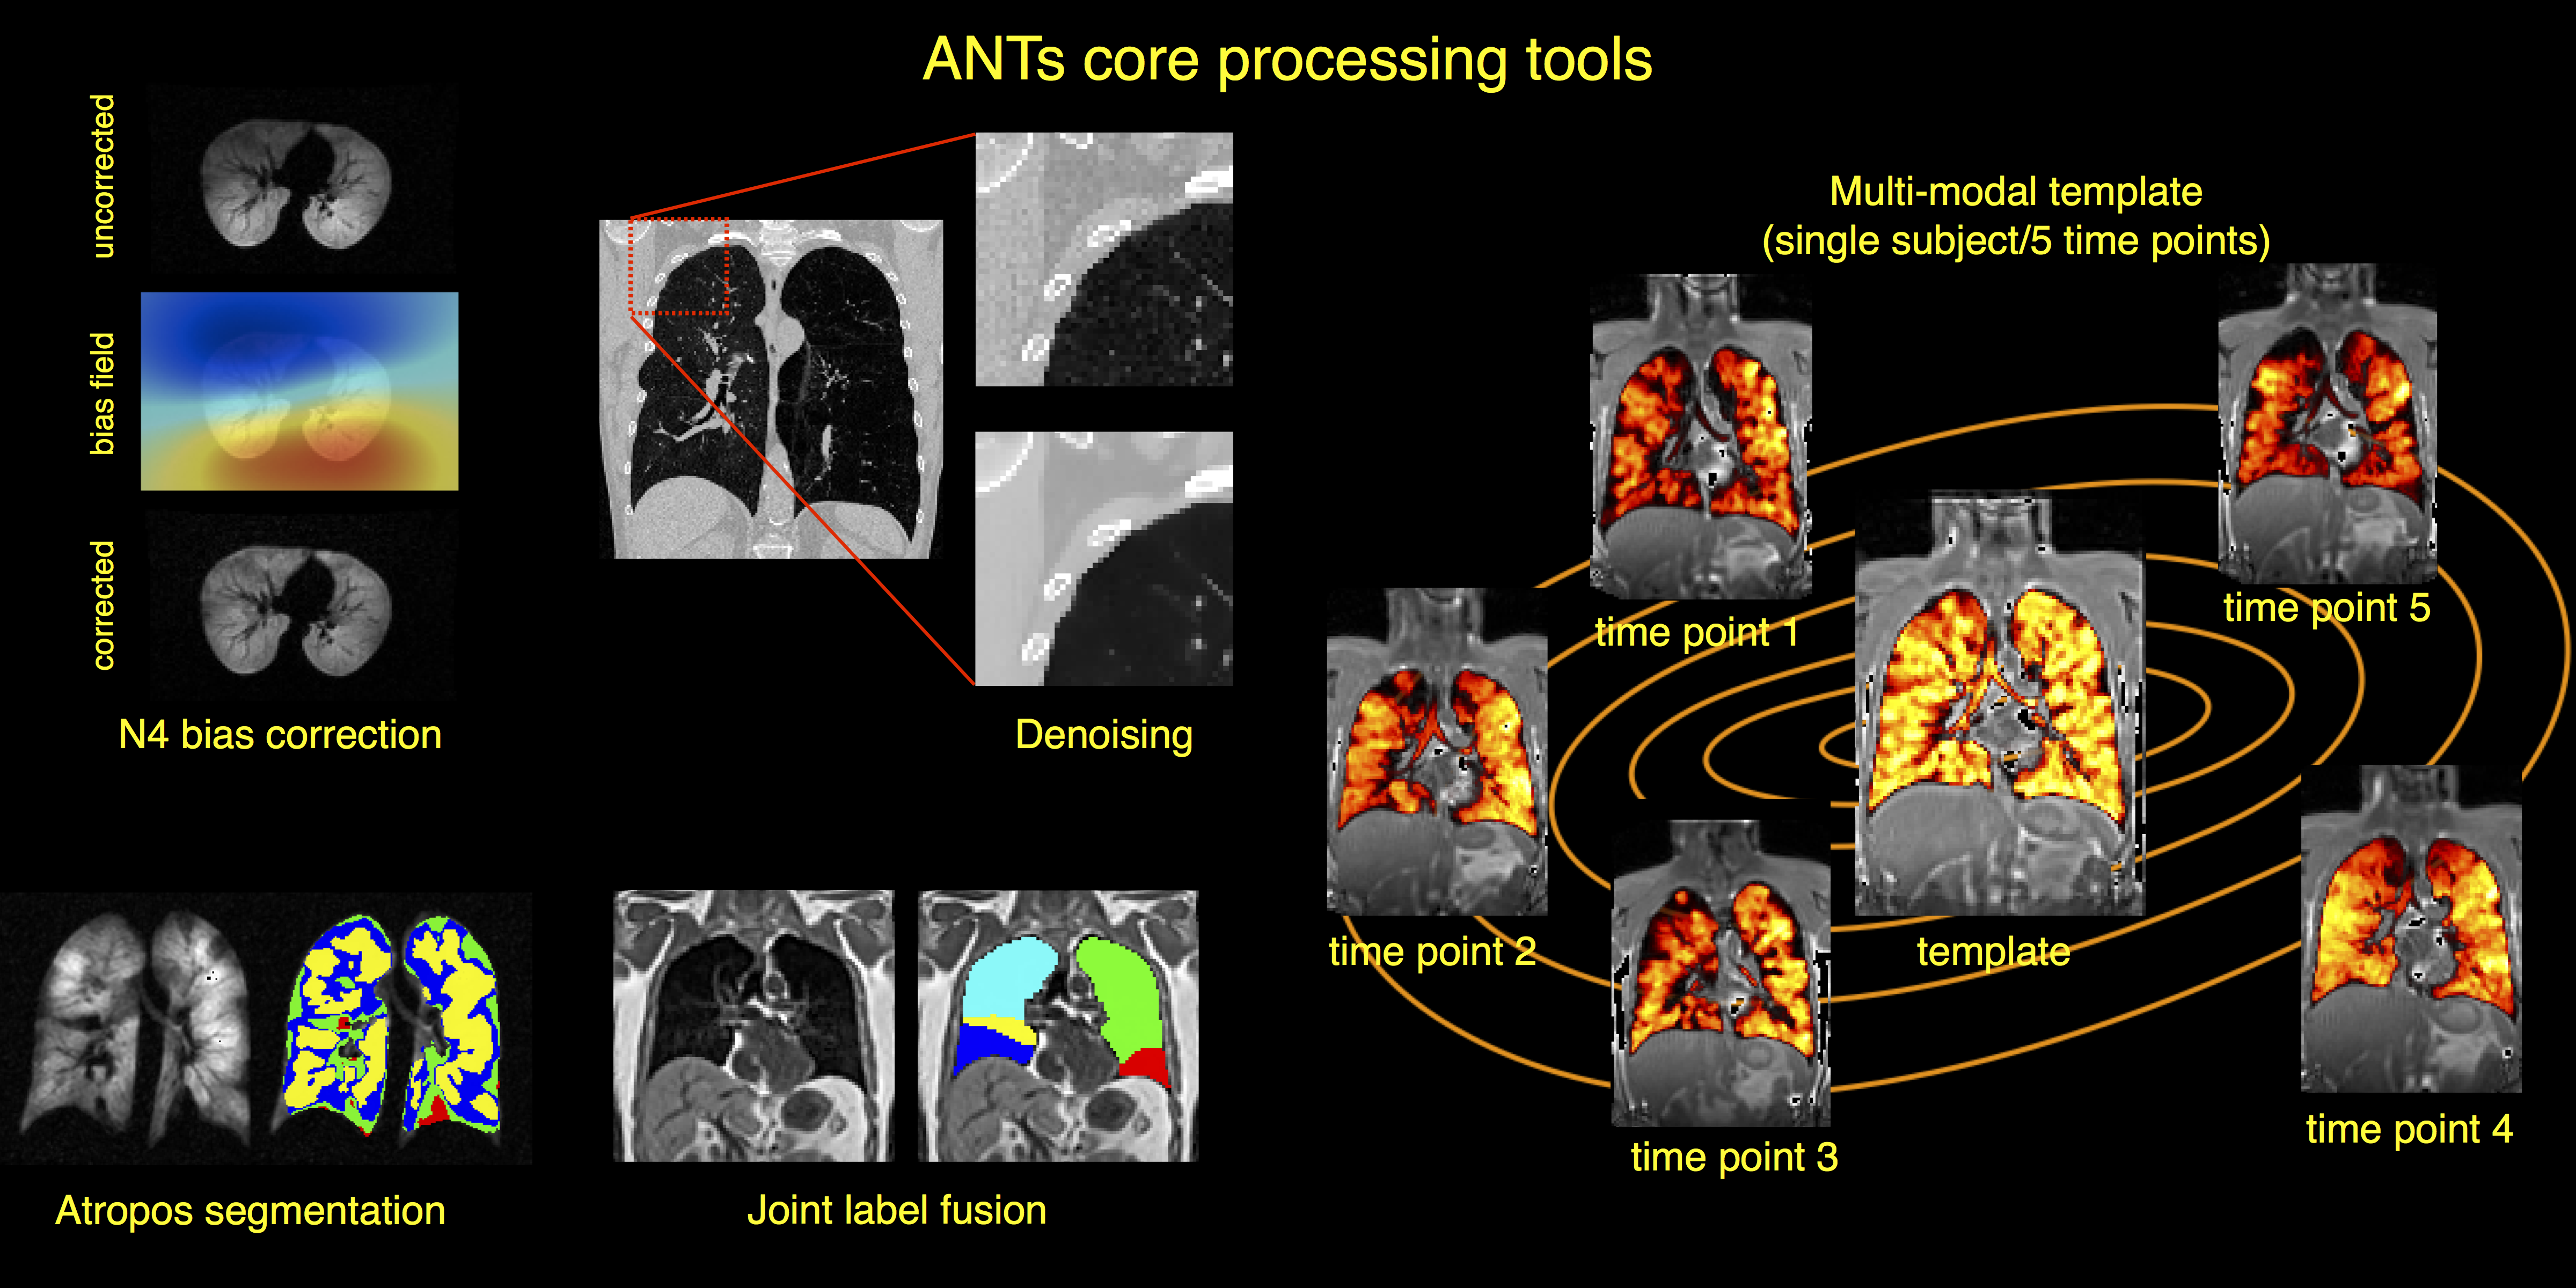
\includegraphics{./tools/figures/coreANtsToolsLung.png}

\end{frame}

\begin{frame}{Symmetric Normalization (SyN)}

\(\int_{t=0}^{0.5} \left(\|\mathbf{v}_1(x,t)\|_L^2 + \|\mathbf{v}_2(x,t)\|_L^2\right)dt + \|I\left(\phi_1(x,0.5)\right) - J_i\left(\phi_2(x,0.5)\right)\|^2\)

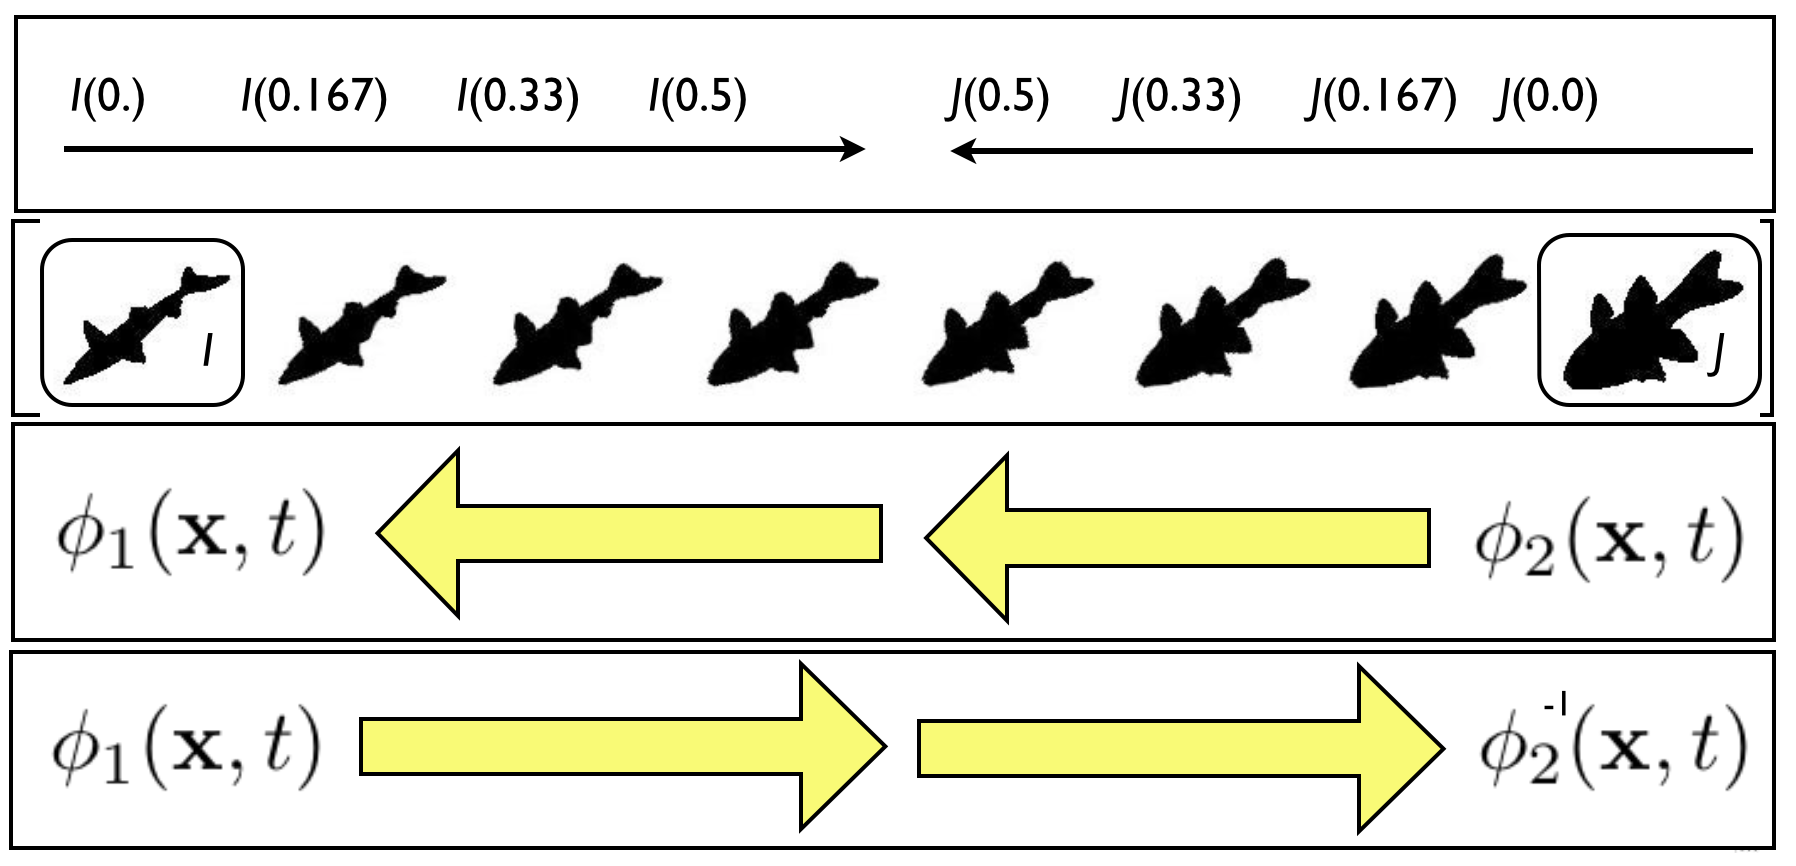
\includegraphics{./papers/figures/fishes.png}

--\textgreater{}

NOtes: * Previously discussed Brians work * The variant most widely used
--\textgreater{}

\end{frame}

\begin{frame}{Beyond original SyN}

\small


\includegraphics{./papers/figures/Frontiers_ITK.png}

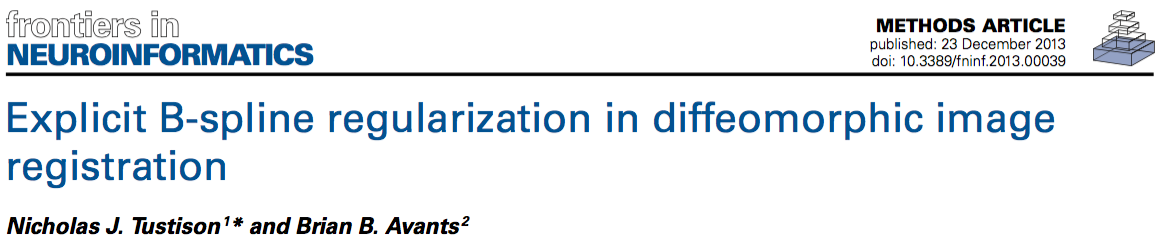
\includegraphics{./papers/figures/Frontiers_BSplineSyN.png}

\end{frame}

\begin{frame}{Nonparametric nonuniform intensity normalization (N3)}

\begin{itemize}
\item
  Developed at the Montreal Neurological Institute (John Sled, 1998)
\item
  Part of the standard preprocessing protocol in large scale projects
  such as ADNI
\item
  The traditional de facto standard in MRI bias correction

  \begin{itemize}
  \tightlist
  \item
    good performance
  \item
    \emph{public availability}
  \end{itemize}
\item
  Public availability --- set of perl scripts coordinating various C++
  programs
\item
  ``\emph{Let's incorporate N3 into ANTs!}''
\end{itemize}

\end{frame}

\begin{frame}{Nonparametric nonuniform intensity normalization (N3)}

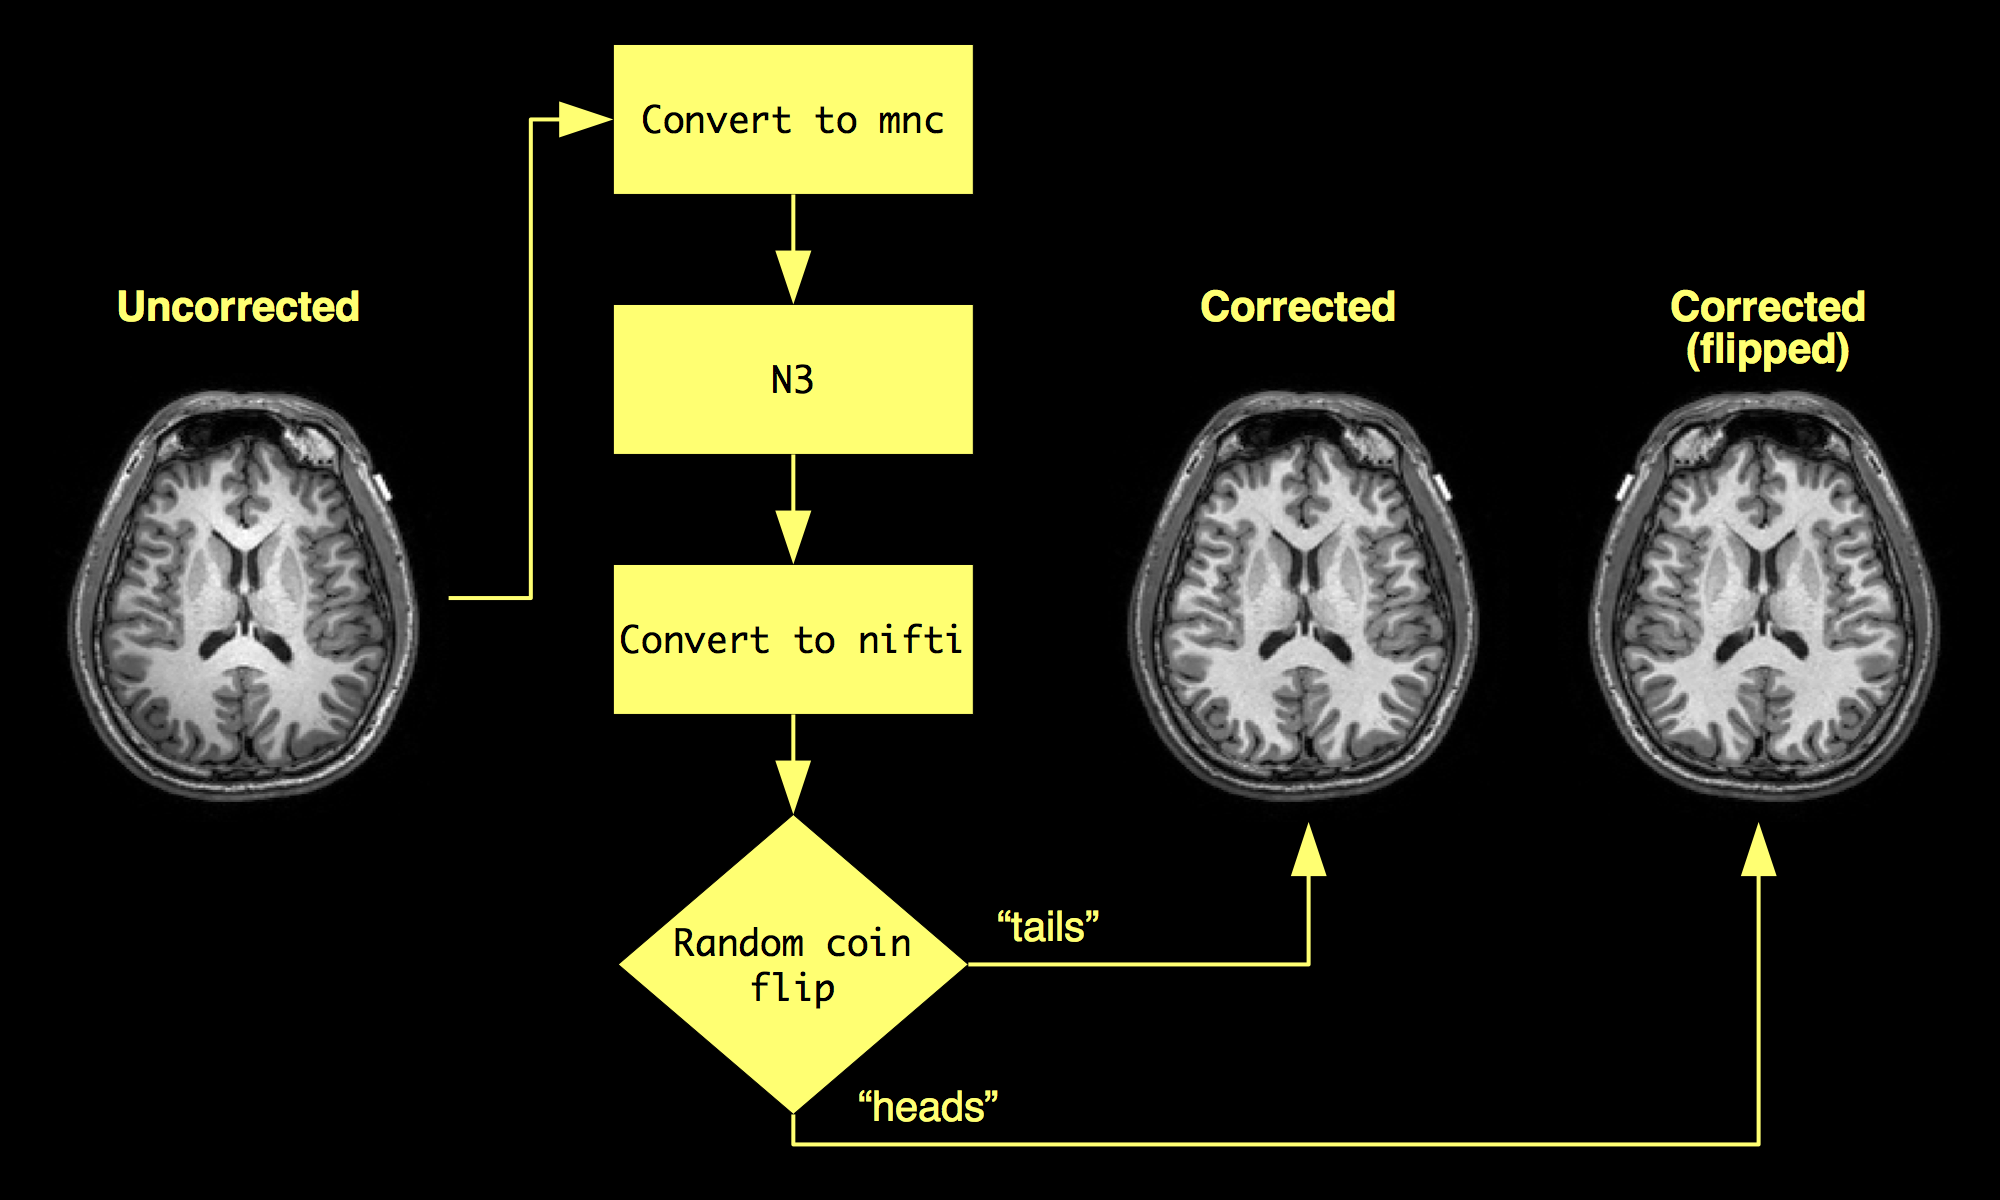
\includegraphics{./tools/n4/figures/whyN4.png}

\end{frame}

\begin{frame}{Atropos: flexible code base}

``20+ years of development. \emph{Show me the code!}''

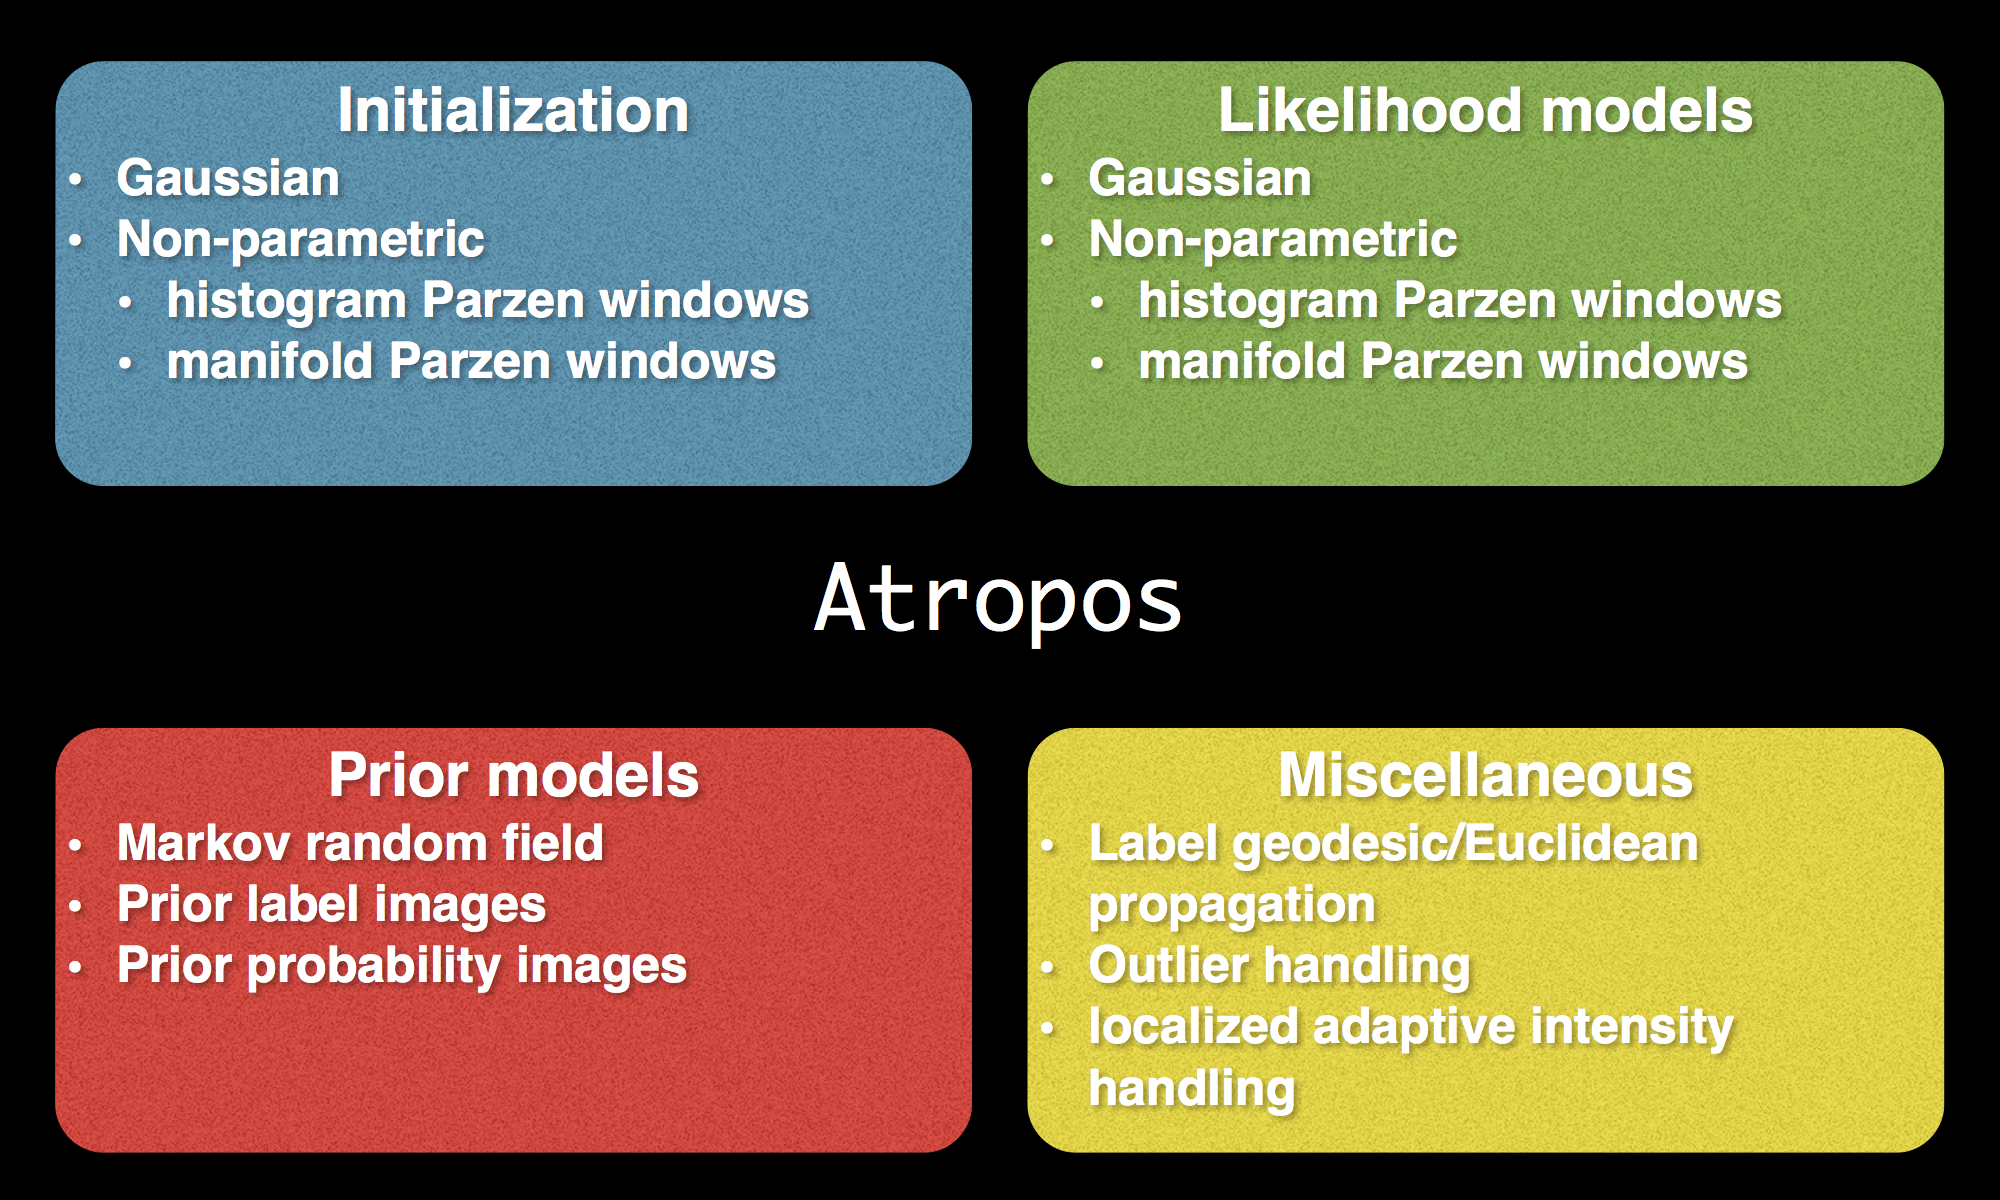
\includegraphics{./tools/atropos/figures/atropos.png}

\end{frame}

\begin{frame}{Atropos + N4 \(\rightarrow\) \texttt{antsAtroposN4.sh}}

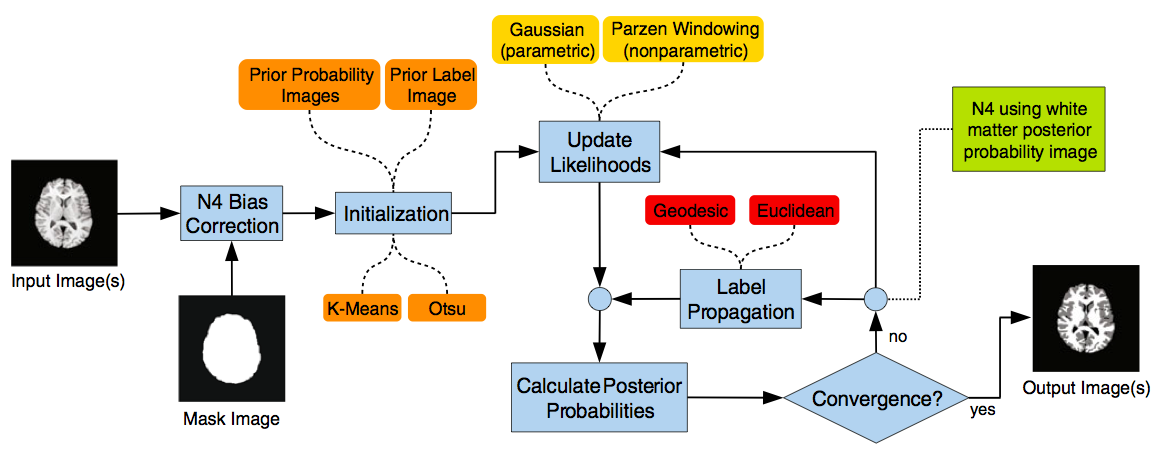
\includegraphics{./tools/atropos/figures/atroposFlow.png}

\end{frame}

\begin{frame}{\texttt{DenoiseImage} --- contribution from Jose Manjon}

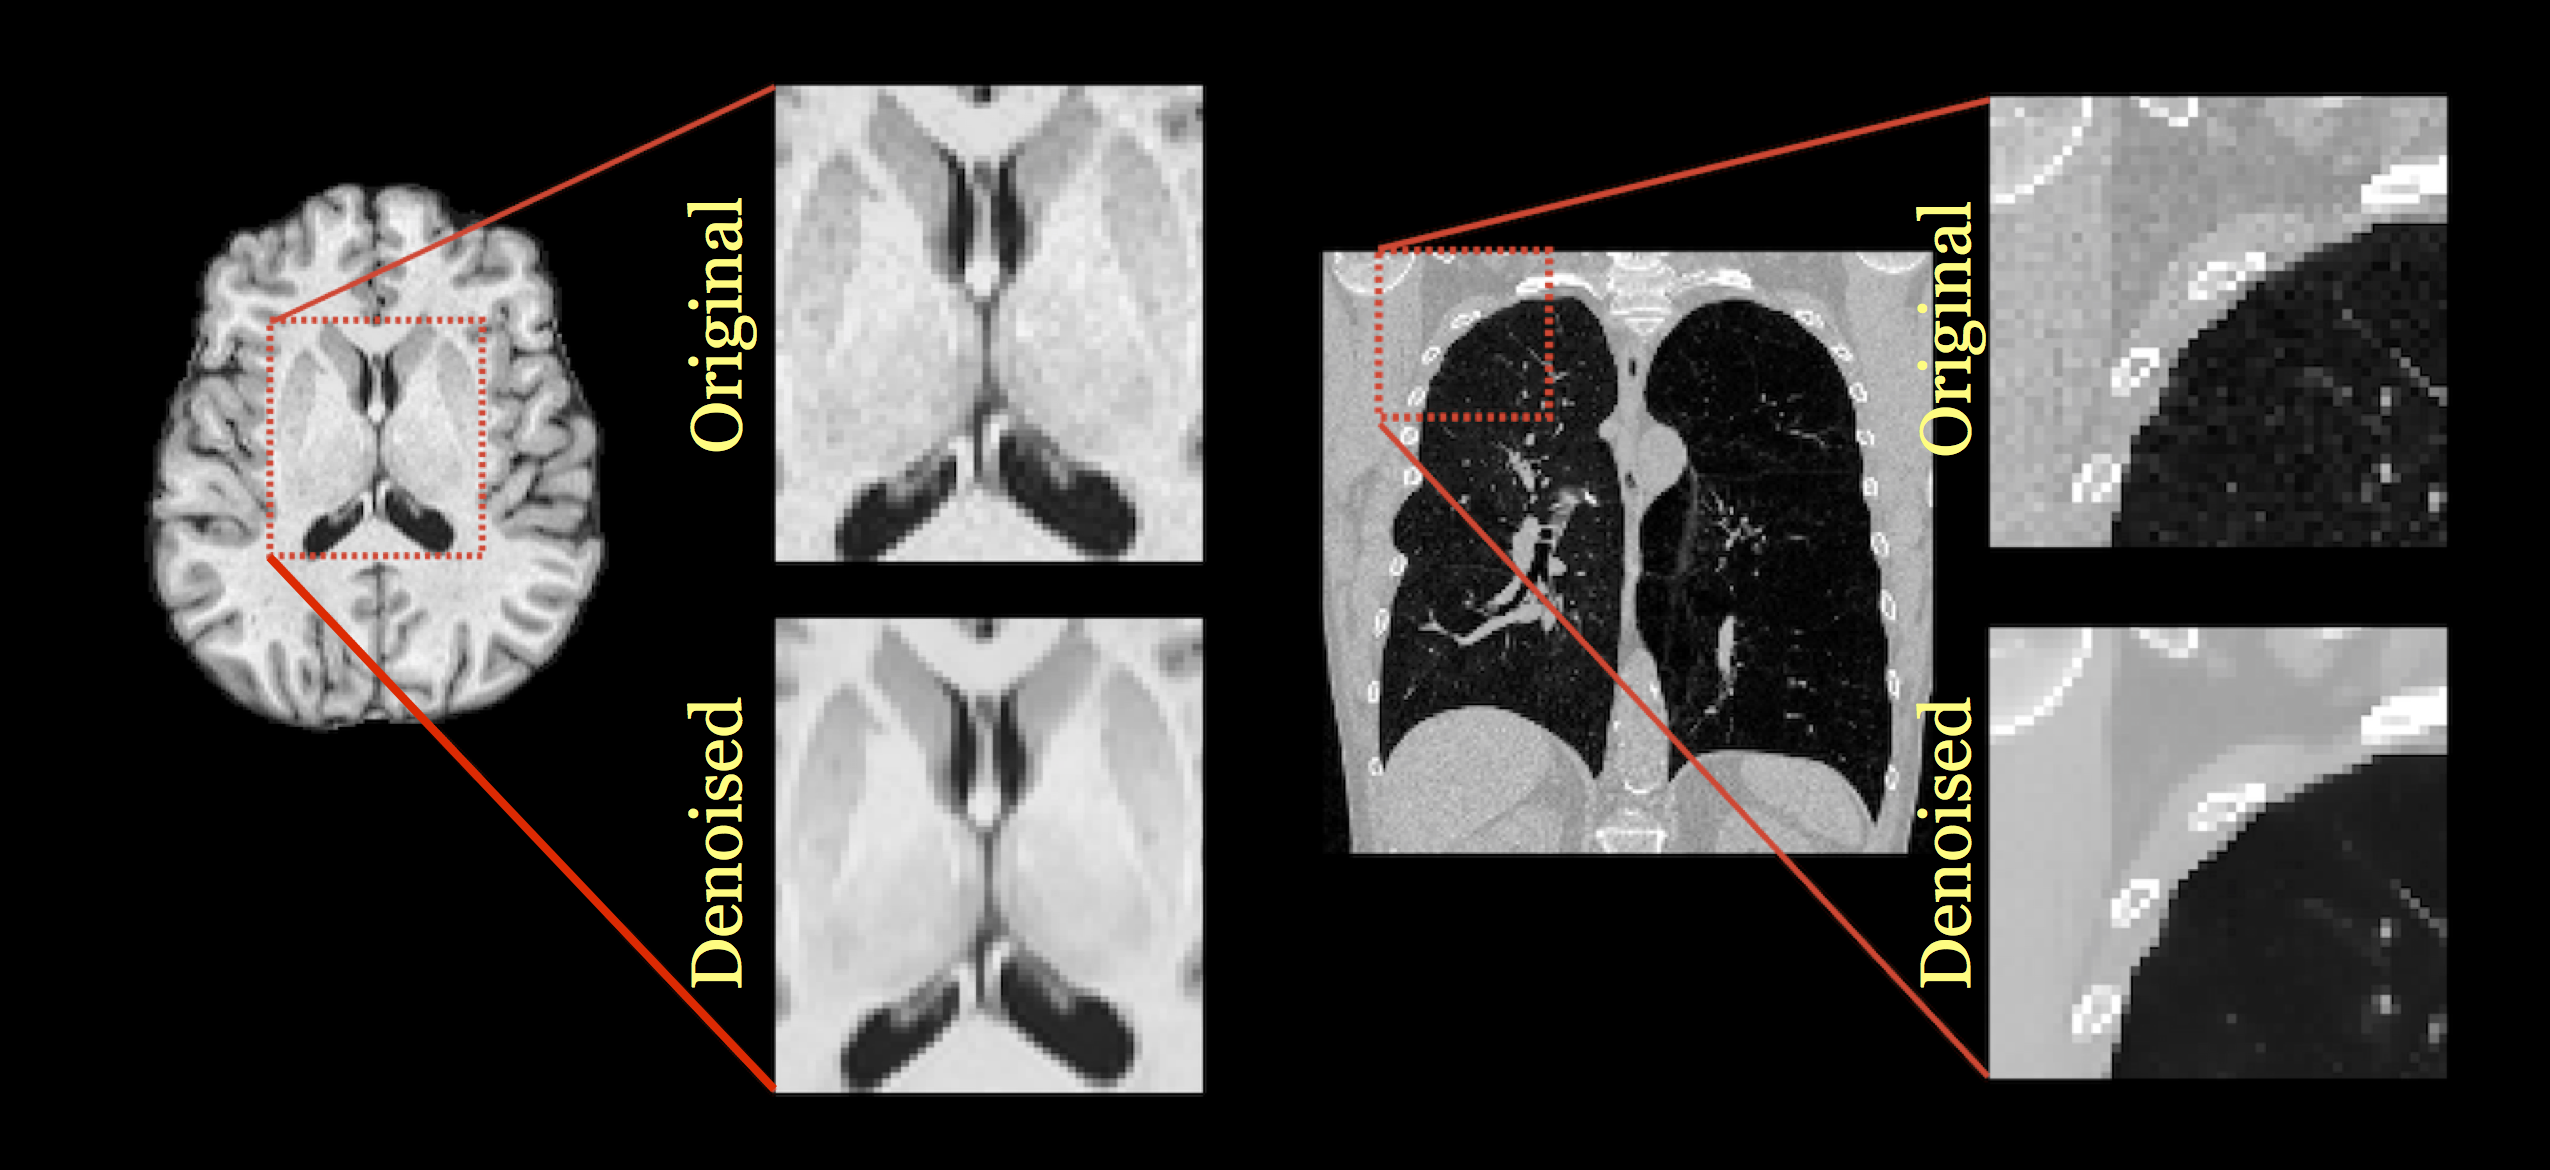
\includegraphics{./tools/figures/denoising.png}

\end{frame}

\begin{frame}{Multi-atlas segmentation}

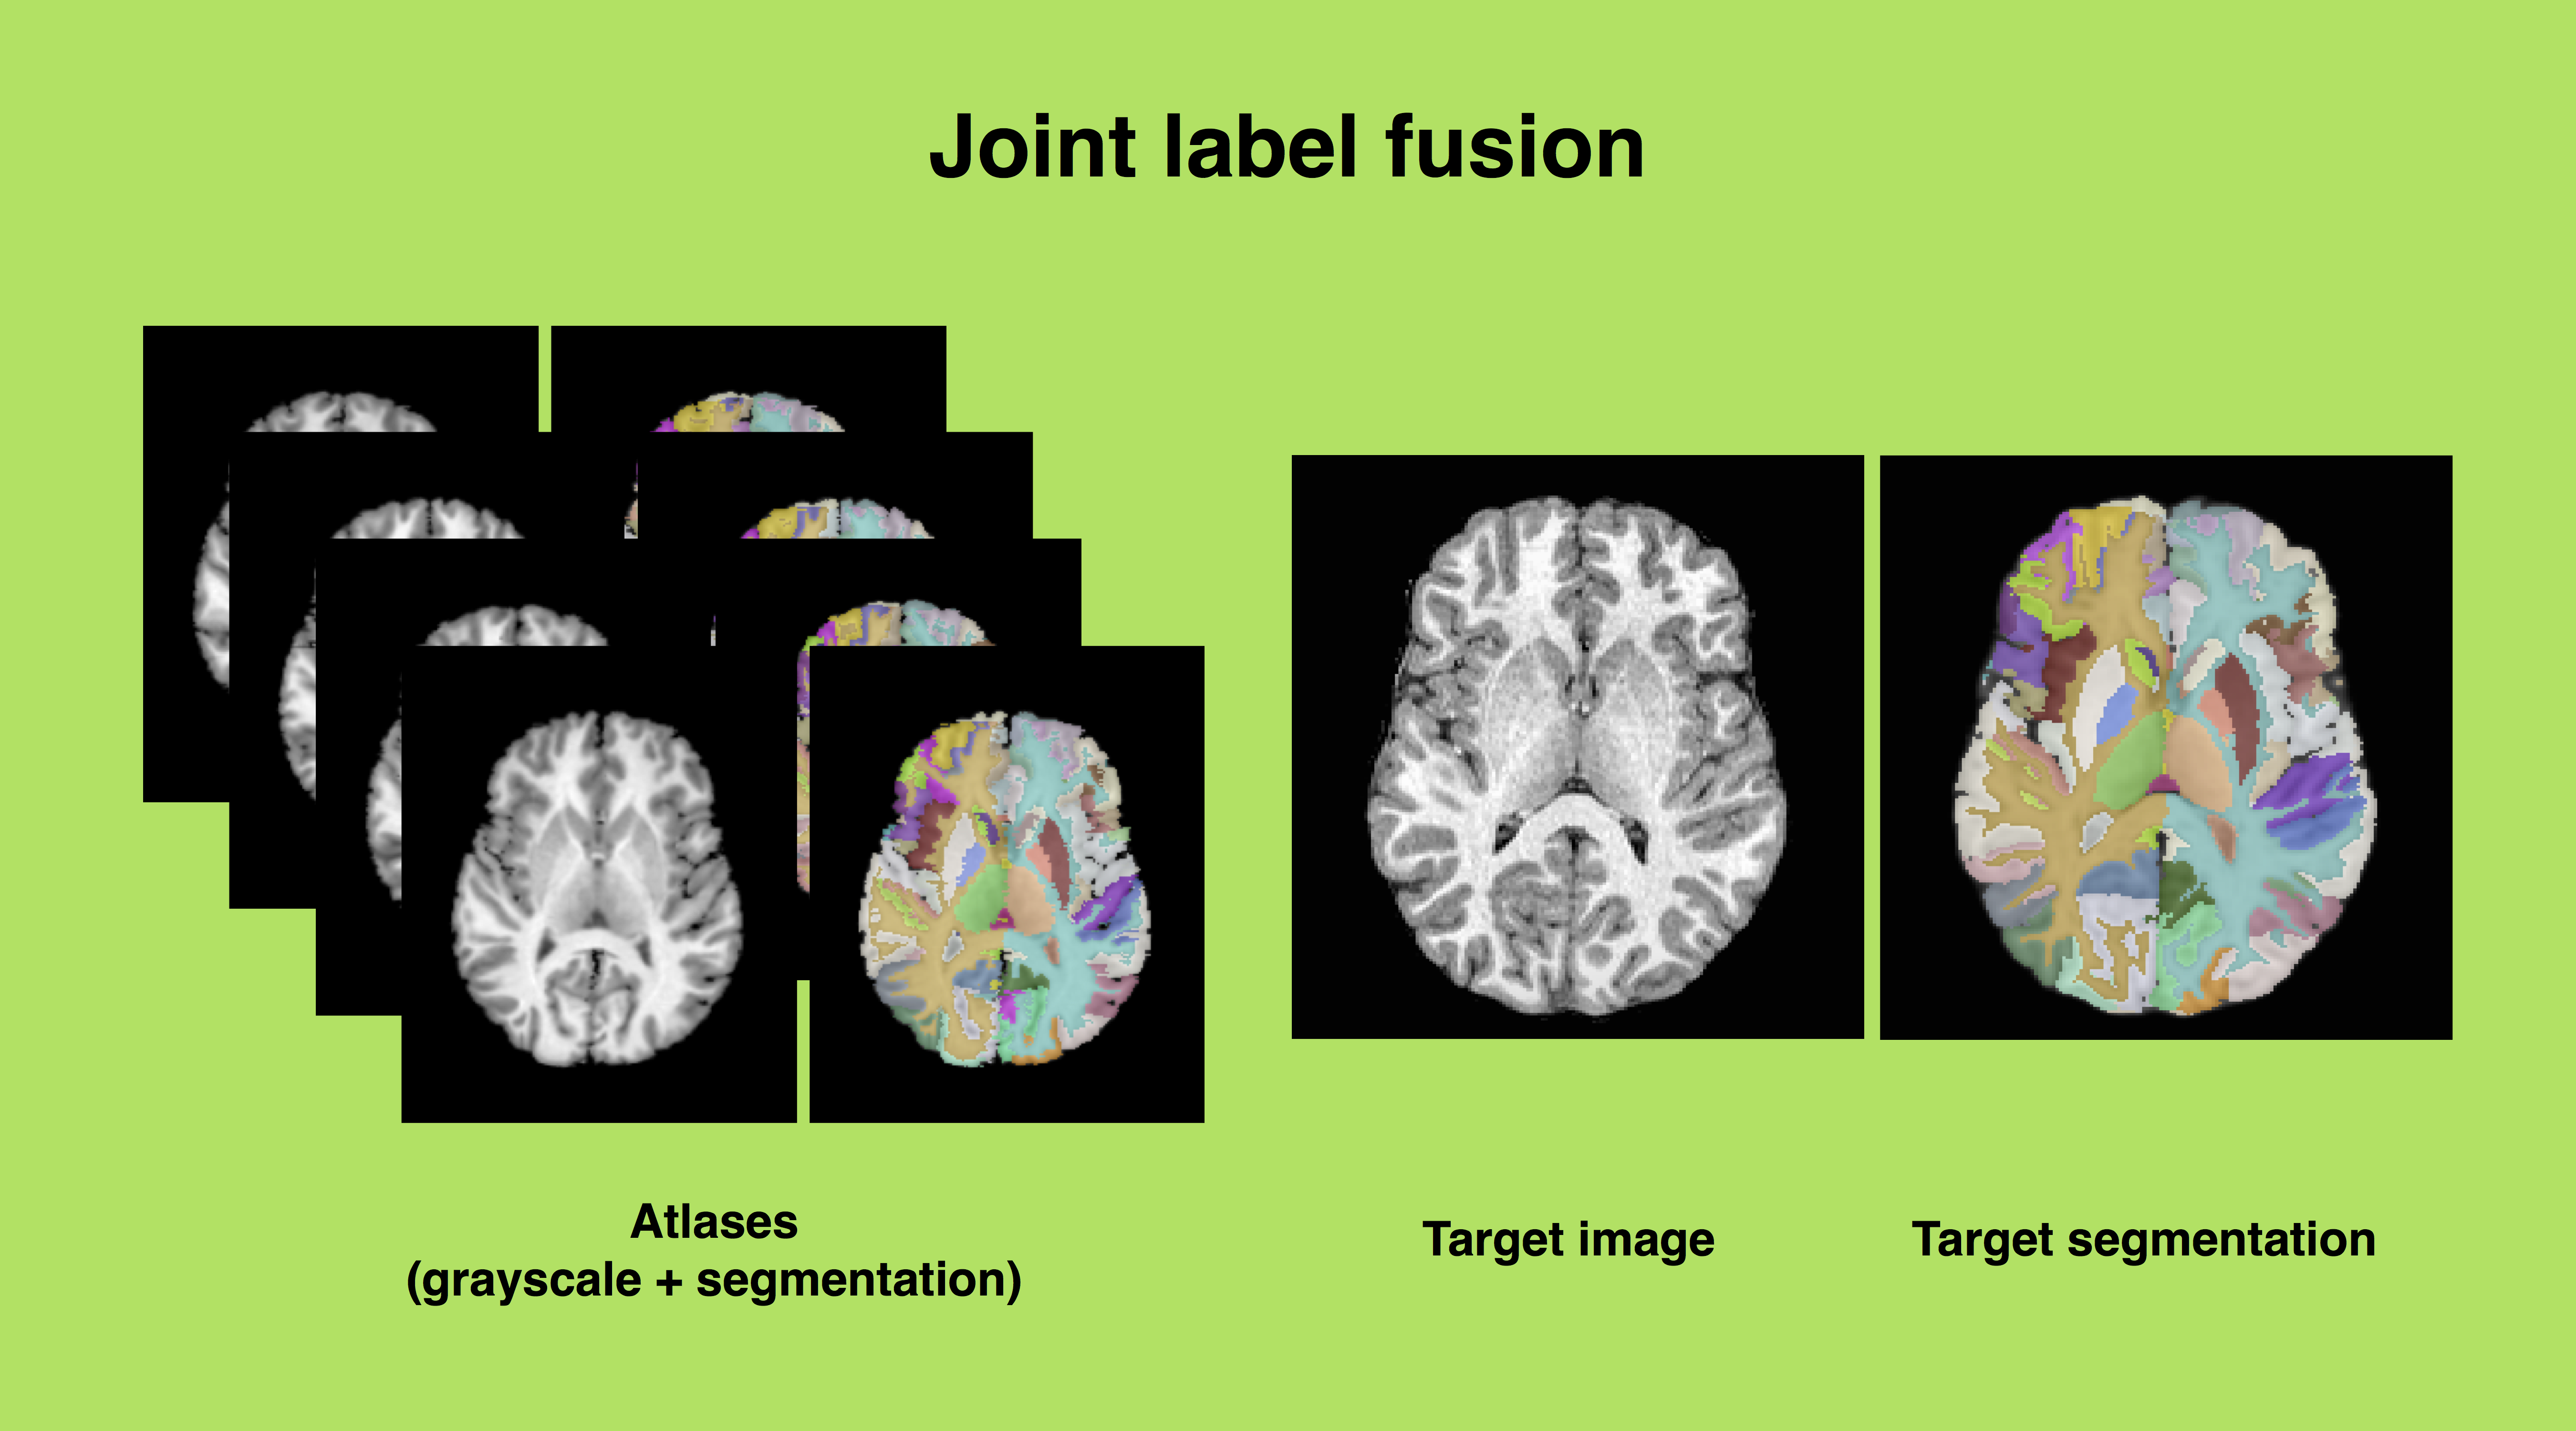
\includegraphics{./tools/jointfusion/figures/jointLabelFusion.png}

\end{frame}

\begin{frame}{New work: joint intensity fusion}

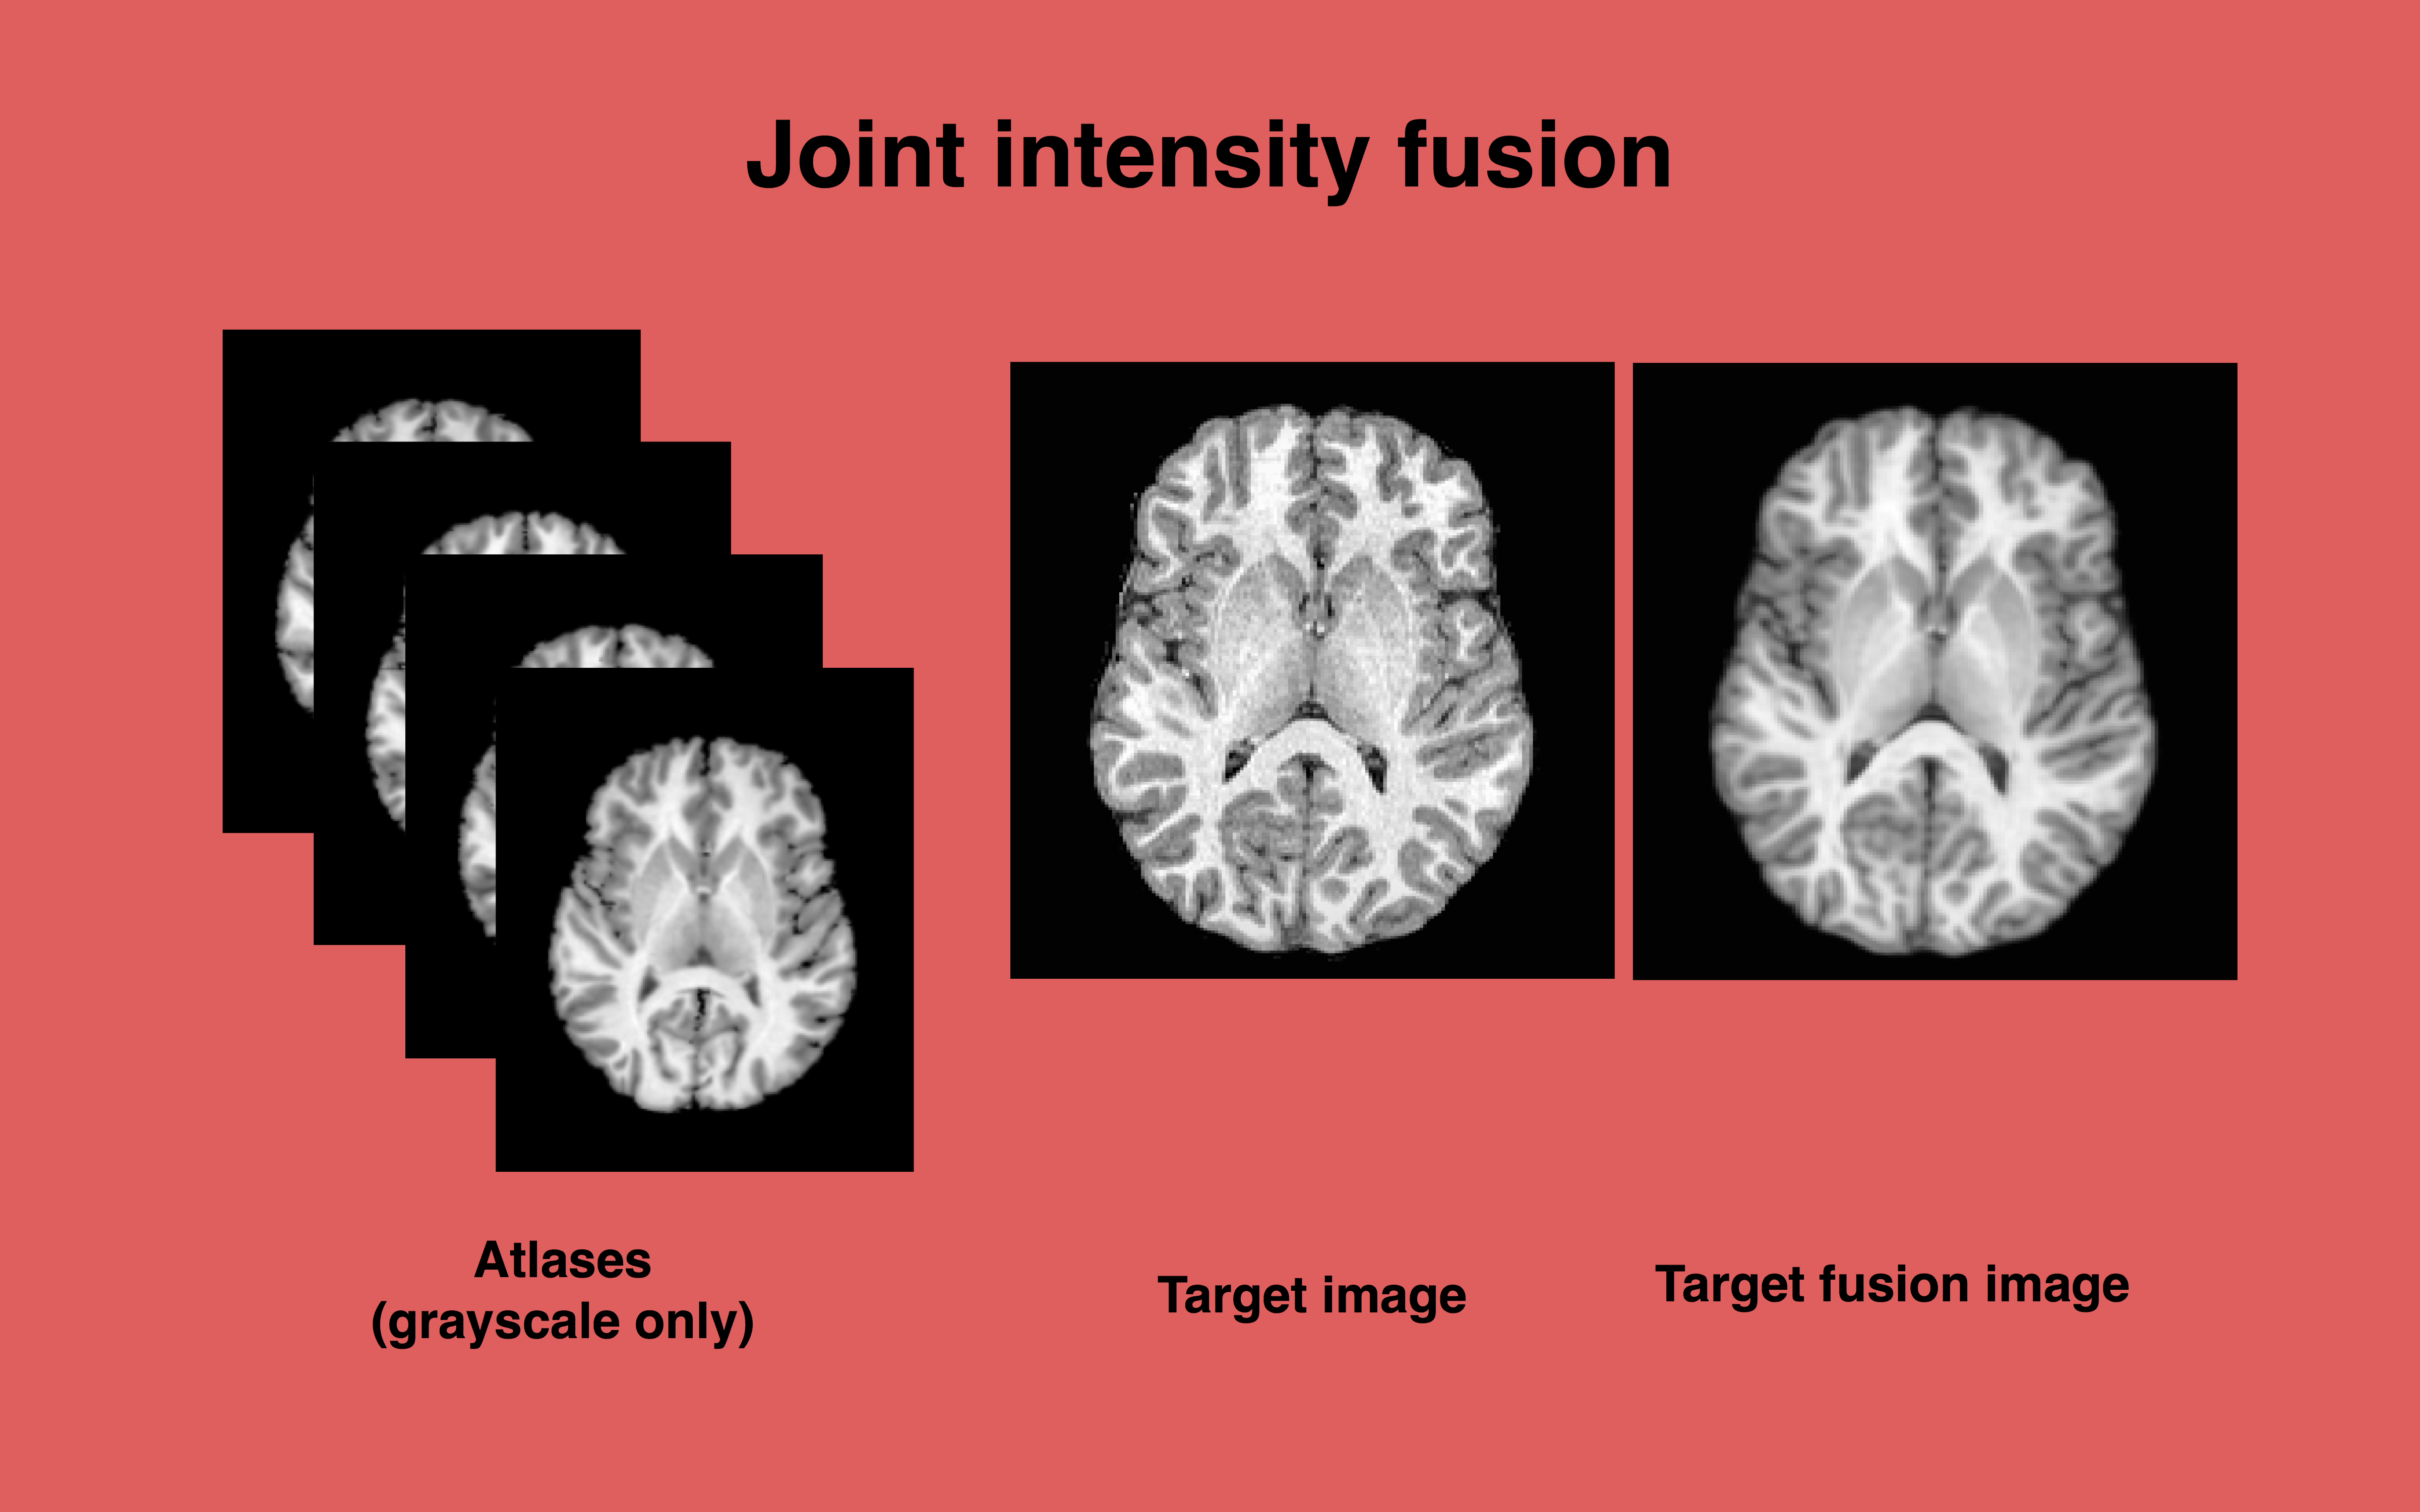
\includegraphics{./tools/jointfusion/figures/jointIntensityFusion.png}

\end{frame}

\section{Putting it all together---the ANTs cortical thickness
pipeline}\label{putting-it-all-togetherthe-ants-cortical-thickness-pipeline}

\begin{frame}{Cortical thickness studies}

\begin{longtable}[c]{@{}ll@{}}
\toprule
Column1 & Column2\tabularnewline
\midrule
\endhead
Tetris-playing ability & chronic pancreatitis\tabularnewline
Huntington's disease & obsessive-compulsive disorder\tabularnewline
schizophrenia & ADHD\tabularnewline
bipolar disorder & obesity\tabularnewline
Alzheimer's disease & heritable depression\tabularnewline
frontotemporal dementia & elderly depression\tabularnewline
Parkinson's disease & age\tabularnewline
Williams syndrome & gender\tabularnewline
multiple sclerosis & handedness\tabularnewline
autism & intelligence\tabularnewline
migraines & athletic ability\tabularnewline
chronic smoking & meditative practices\tabularnewline
alcoholism & musical ability\tabularnewline
cocaine addiction & tendency toward criminality\tabularnewline
Tourette syndrome in children & childhood sexual abuse in female
adolescents\tabularnewline
scoliosis in female adolescents & traumatic brain injury\tabularnewline
early-onset blindness & untreated male-to-female
transsexuality\tabularnewline
\bottomrule
\end{longtable}

\end{frame}

\begin{frame}{The ANTs structural brain mapping workflow}

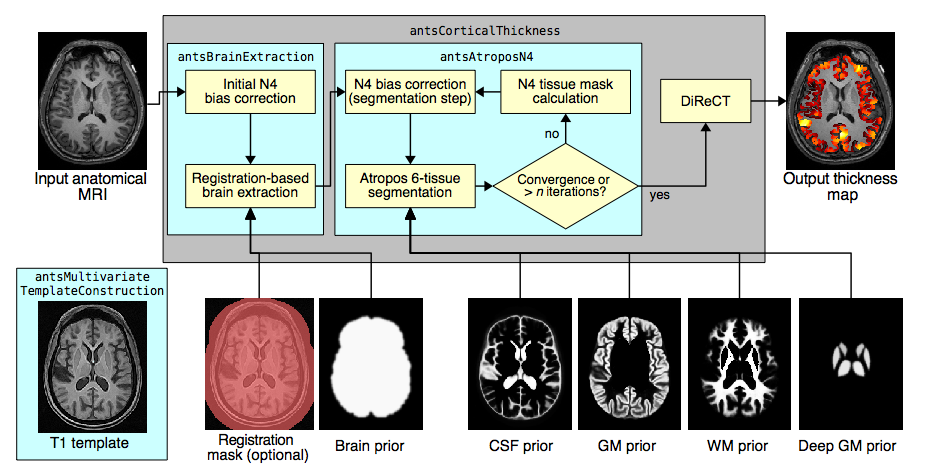
\includegraphics{./evaluation/figures/pipeline.png}

\end{frame}

\begin{frame}{Template building}

\emph{Tailor data to your specific cohort}

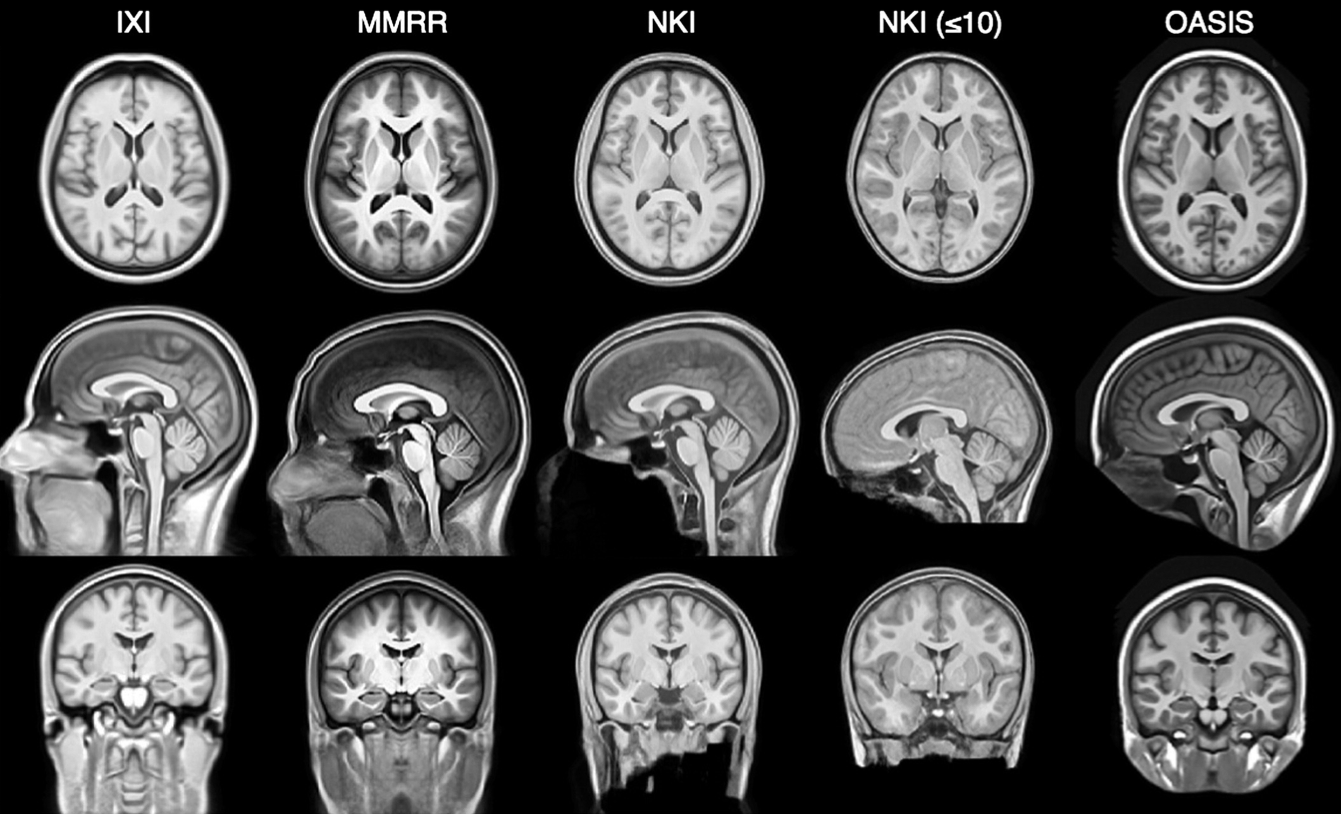
\includegraphics{./evaluation/figures/templates.png}

\begin{itemize}
\tightlist
\item
  Templates representing the average mean shape and intensity are built
  directly from the
\item
  cohort to be analyzed, e.g.~pediatric vs.~middle-aged brains.
\item
  Acquisition and anonymization (e.g.~defacing) protocols are often
  different.
\end{itemize}

\end{frame}

\begin{frame}{Template priors}

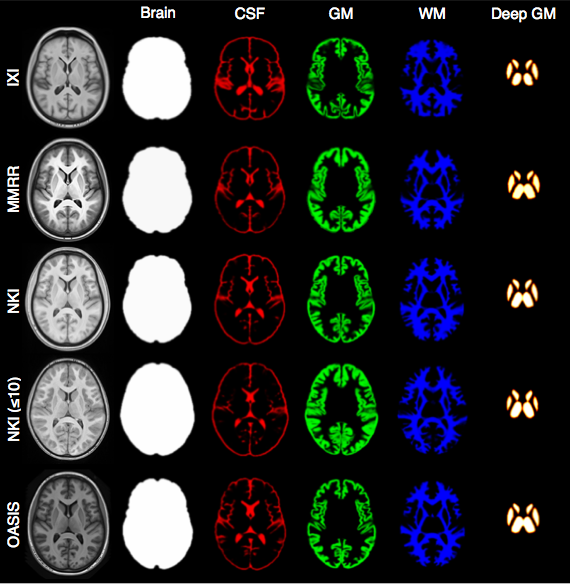
\includegraphics{./evaluation/figures/templatePriors.png}

Each template is
\href{https://github.com/ntustison/antsCookTemplatePriorsExample}{processed}
to produce auxiliary images which are used for brain extraction and
brain segmentation.

\end{frame}

\begin{frame}{Brain extraction comparison}

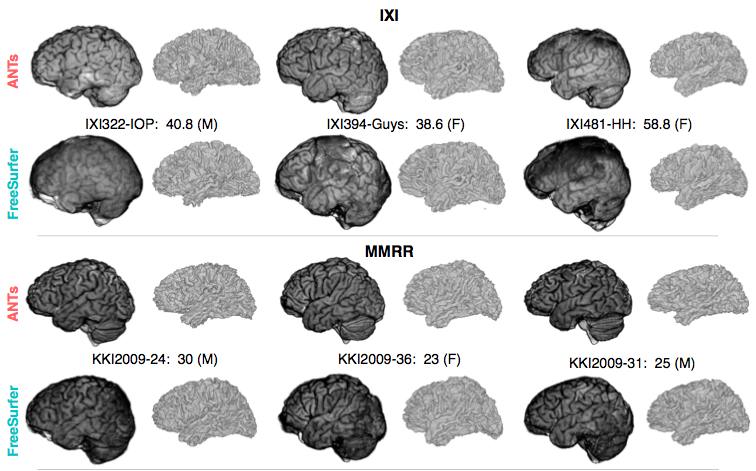
\includegraphics{./evaluation/figures/brainExtraction.png}

Comparison with de facto standard FreeSurfer package. Note the
difference in separation of the gray matter from the surrounding CSF. (0
failures out of 1205 scans)

\end{frame}

\begin{frame}[fragile]{Brain segmentation}

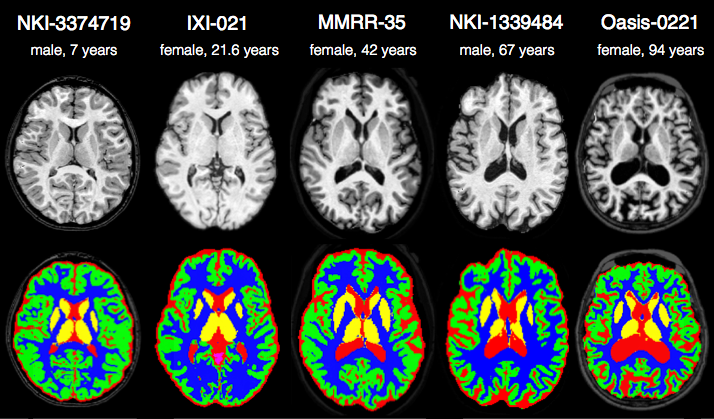
\includegraphics{./evaluation/figures/brainSegmentation.png}

Randomly selected healthy individuals. \texttt{Atropos} gets good
performance across ages.

\end{frame}

\begin{frame}{Cortical thickness maps}

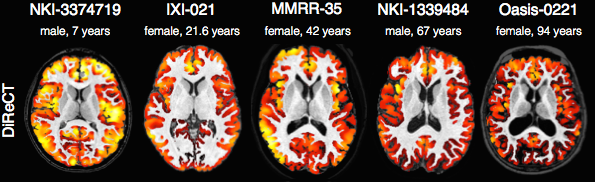
\includegraphics{./evaluation/figures/corticalThicknessEstimation.png}

In contrast to FreeSurfer which warps coupled surface meshes to segment
the gray matter, \emph{ANTs} diffeomorphically registers the white
matter to the combined gray/white matters while simultaneously
estimating thickness.

\end{frame}

\begin{frame}

\emph{But without ground truth, how does one evaluate the pipeline?}

\end{frame}

\begin{frame}{Predict age and gender}

\(AGE \sim VOLUME + GENDER + \sum_{i=1}^{62} T(DKT_i)\)

\end{frame}

\begin{frame}{Open science principles}

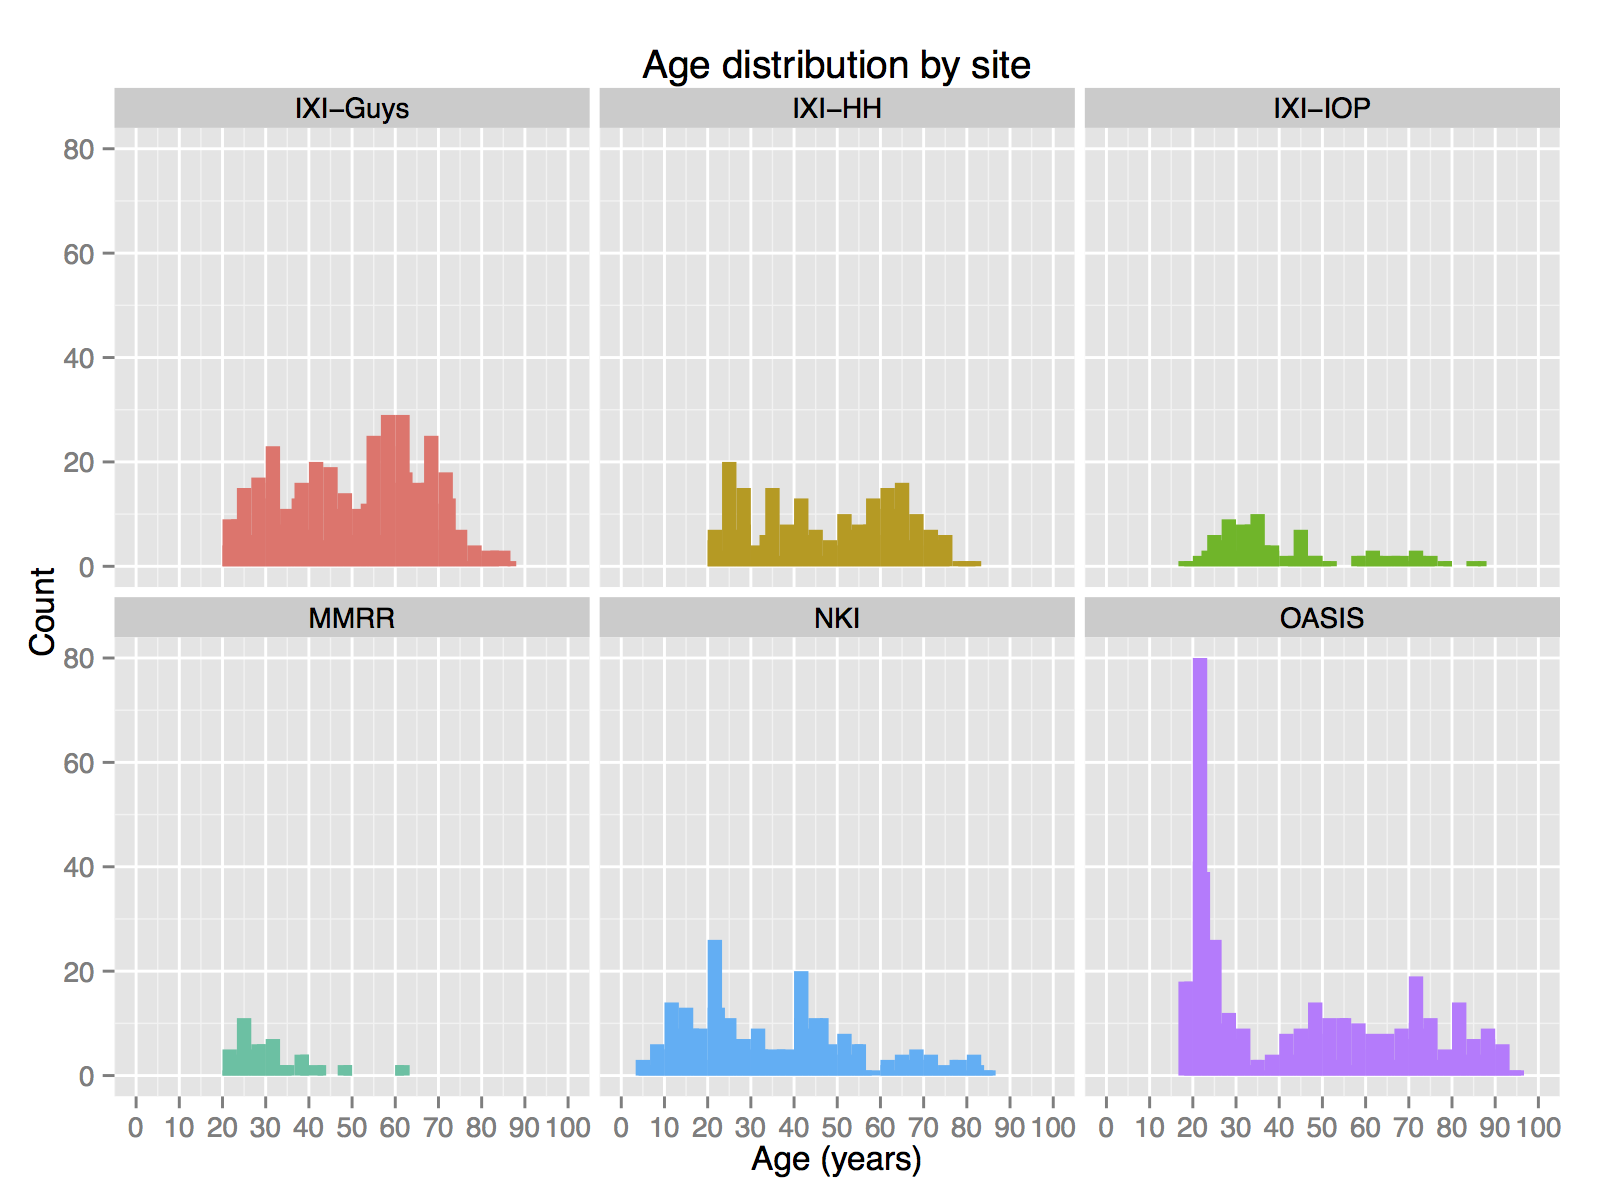
\includegraphics{./evaluation/figures/ageDistribution.png}

\begin{itemize}
\tightlist
\item
  Public data sets (IXI, NKI, OASIS, MMRR)
\item
  \(>\) 1200 subjects, age 4 to over 94 years old
\end{itemize}

\end{frame}

\begin{frame}{Prediction from cortical thickness data}

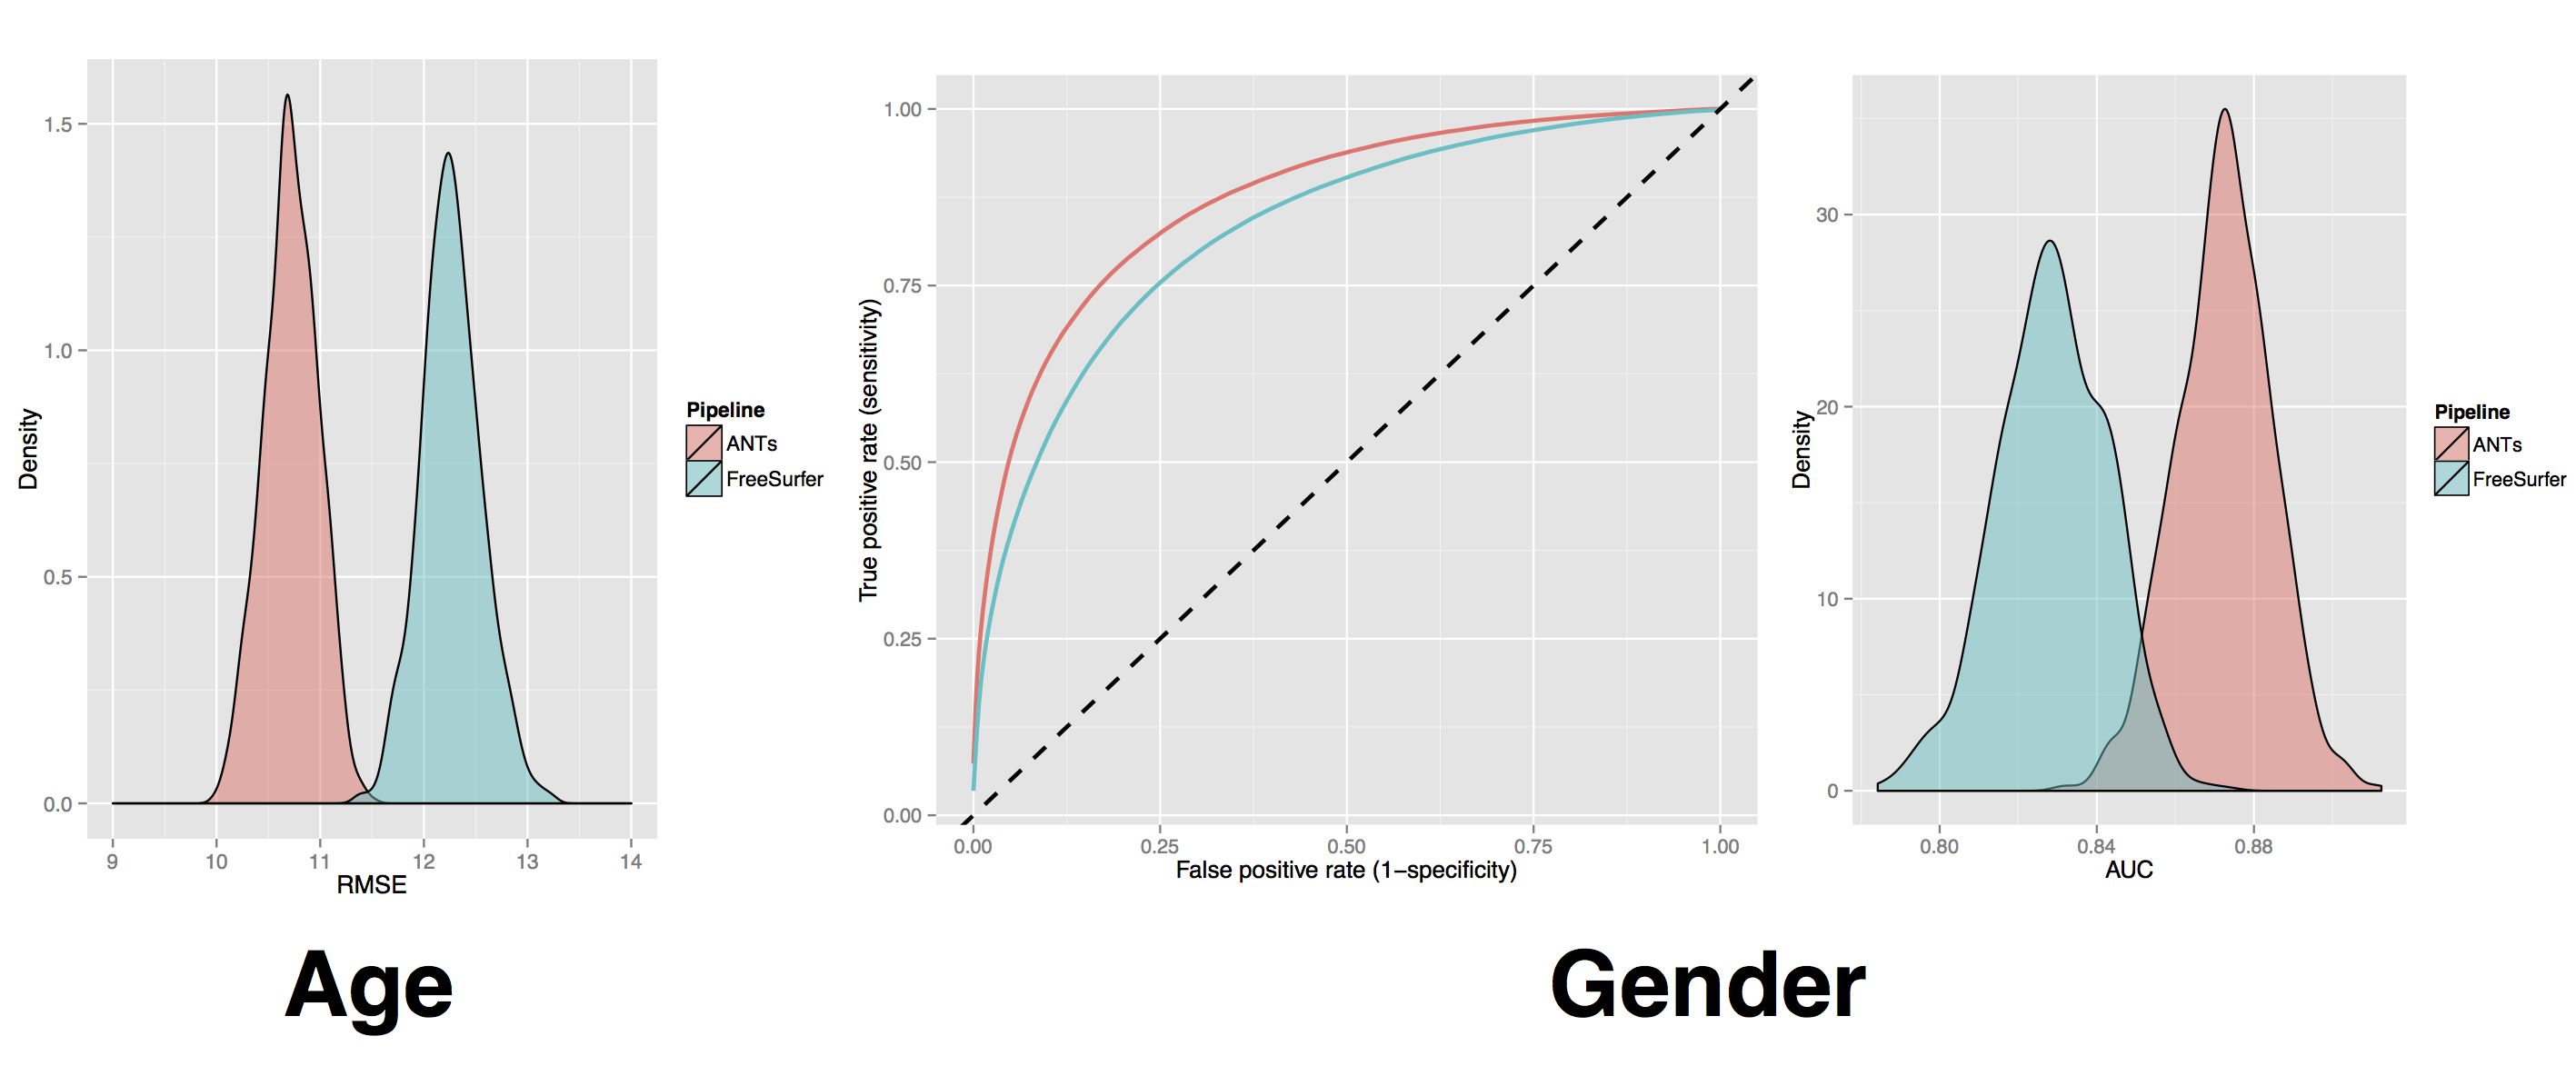
\includegraphics{./evaluation/figures/evaluation.png}

\end{frame}

\begin{frame}{Age prediction per site}

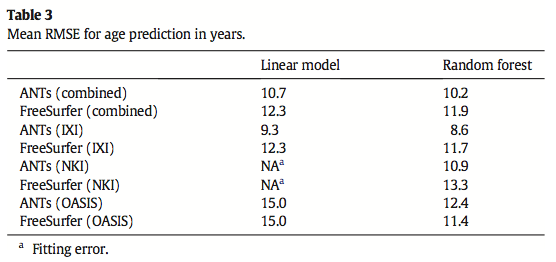
\includegraphics{./evaluation/figures/agePredictionPerSite.png}

\end{frame}

\begin{frame}{Regional importance comparison}

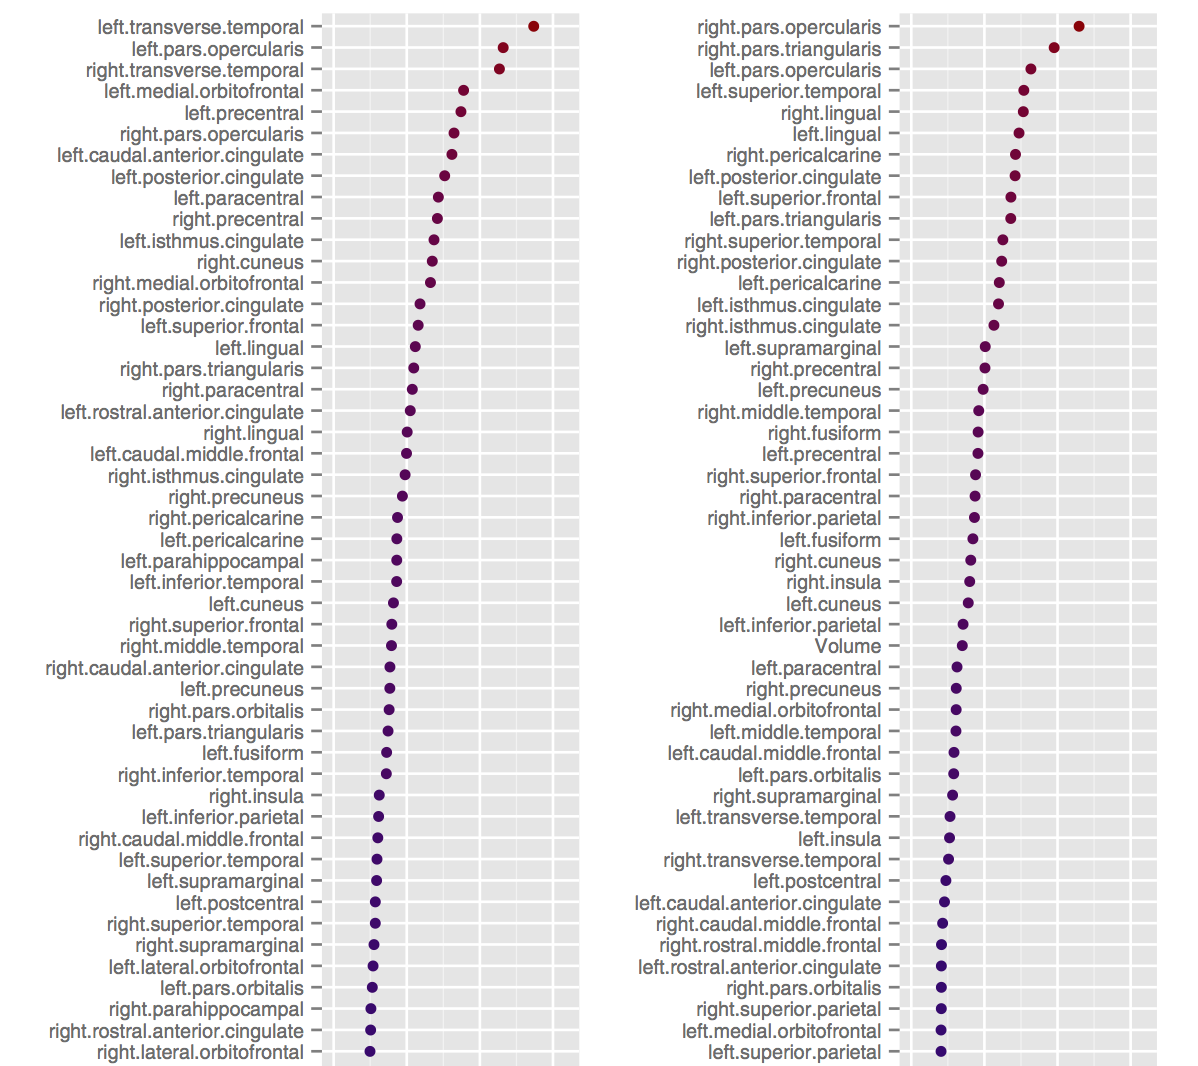
\includegraphics{./evaluation/figures/antsvfreesurfer_Importance.png}

ANTs (left) vs.~FreeSurfer (right)

\end{frame}

\begin{frame}{Regional measurements}

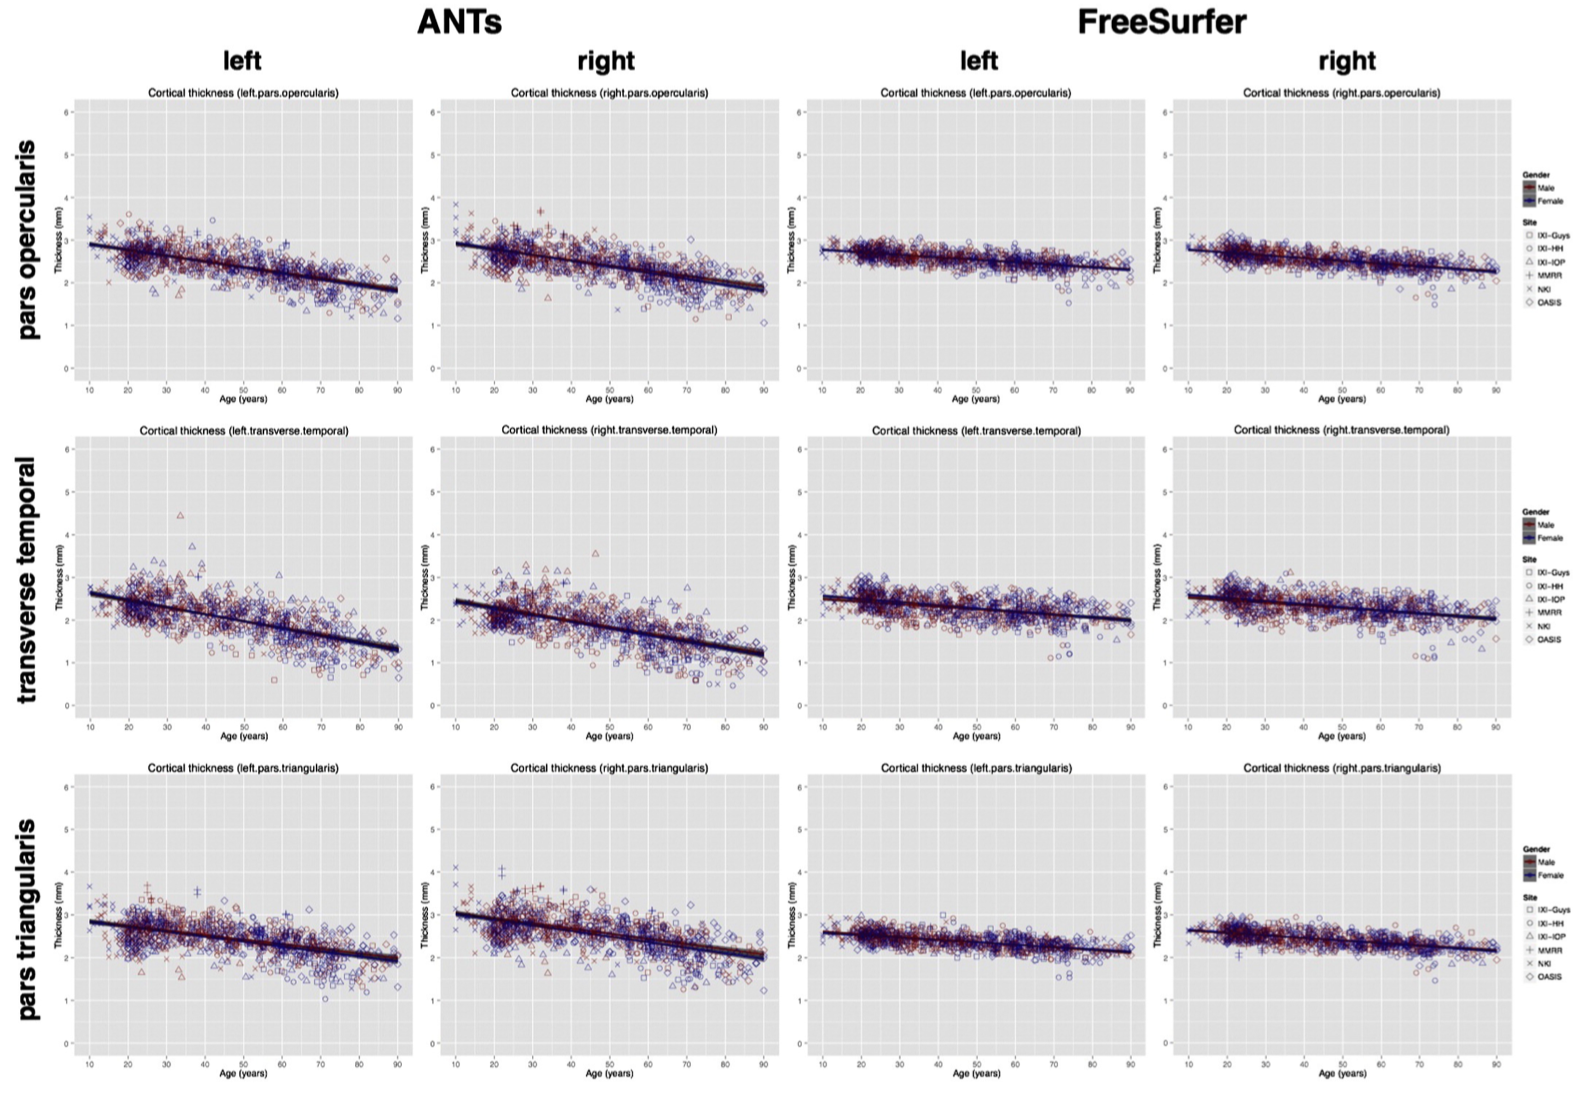
\includegraphics{./evaluation/figures/antsvfreesurfer_regionalPlots.png}

\hypertarget{refs}{}

\end{frame}

\end{document}
